\documentclass[12pt,]{article}
%DIF LATEXDIFF DIFFERENCE FILE
%DIF DEL LMAps_main.tex      Thu Jun 14 11:32:29 2018
%DIF ADD LMAps_main_re.tex   Thu Jun 14 11:32:36 2018
\usepackage{lmodern}
\usepackage{amssymb,amsmath}
\usepackage{ifxetex,ifluatex}
\usepackage{fixltx2e} % provides \textsubscript
\ifnum 0\ifxetex 1\fi\ifluatex 1\fi=0 % if pdftex
  \usepackage[T1]{fontenc}
  \usepackage[utf8]{inputenc}
\else % if luatex or xelatex
  \ifxetex
    \usepackage{mathspec}
  \else
    \usepackage{fontspec}
  \fi
  \defaultfontfeatures{Ligatures=TeX,Scale=MatchLowercase}
%DIF 16d16
%DIF <     \setsansfont[]{Times New Roman}
%DIF -------
\fi
% use upquote if available, for straight quotes in verbatim environments
\IfFileExists{upquote.sty}{\usepackage{upquote}}{}
% use microtype if available
\IfFileExists{microtype.sty}{%
\usepackage{microtype}
\UseMicrotypeSet[protrusion]{basicmath} % disable protrusion for tt fonts
}{}
\usepackage[margin=1in]{geometry}
\usepackage{hyperref}
\hypersetup{unicode=true,
            pdfborder={0 0 0},
            breaklinks=true}
\urlstyle{same}  % don't use monospace font for urls
\usepackage{longtable,booktabs}
\usepackage{graphicx,grffile}
\makeatletter
\def\maxwidth{\ifdim\Gin@nat@width>\linewidth\linewidth\else\Gin@nat@width\fi}
\def\maxheight{\ifdim\Gin@nat@height>\textheight\textheight\else\Gin@nat@height\fi}
\makeatother
% Scale images if necessary, so that they will not overflow the page
% margins by default, and it is still possible to overwrite the defaults
% using explicit options in \includegraphics[width, height, ...]{}
\setkeys{Gin}{width=\maxwidth,height=\maxheight,keepaspectratio}
\IfFileExists{parskip.sty}{%
\usepackage{parskip}
}{% else
\setlength{\parindent}{0pt}
\setlength{\parskip}{6pt plus 2pt minus 1pt}
}
\setlength{\emergencystretch}{3em}  % prevent overfull lines
\providecommand{\tightlist}{%
  \setlength{\itemsep}{0pt}\setlength{\parskip}{0pt}}
\setcounter{secnumdepth}{0}
% Redefines (sub)paragraphs to behave more like sections
\ifx\paragraph\undefined\else
\let\oldparagraph\paragraph
\renewcommand{\paragraph}[1]{\oldparagraph{#1}\mbox{}}
\fi
\ifx\subparagraph\undefined\else
\let\oldsubparagraph\subparagraph
\renewcommand{\subparagraph}[1]{\oldsubparagraph{#1}\mbox{}}
\fi

%%% Use protect on footnotes to avoid problems with footnotes in titles
\let\rmarkdownfootnote\footnote%
\def\footnote{\protect\rmarkdownfootnote}

%%% Change title format to be more compact
\usepackage{titling}

% Create subtitle command for use in maketitle
\newcommand{\subtitle}[1]{
  \posttitle{
    \begin{center}\large#1\end{center}
    }
}

\setlength{\droptitle}{-2em}

  \title{}
    \pretitle{\vspace{\droptitle}}
  \posttitle{}
    \author{}
    \preauthor{}\postauthor{}
    \date{}
    \predate{}\postdate{}

\usepackage{times}
\usepackage{setspace}
\doublespacing
\usepackage{lineno}
\linenumbers
\usepackage{amsmath}
% \usepackage{array}
%DIF 92a91-104
\usepackage{booktabs} %DIF >
\usepackage{longtable} %DIF >
\usepackage{array} %DIF >
\usepackage{multirow} %DIF >
\usepackage[table]{xcolor} %DIF >
\usepackage{wrapfig} %DIF >
\usepackage{float} %DIF >
\usepackage{colortbl} %DIF >
\usepackage{pdflscape} %DIF >
\usepackage{tabu} %DIF >
\usepackage{threeparttable} %DIF >
\usepackage{threeparttablex} %DIF >
\usepackage[normalem]{ulem} %DIF >
\usepackage{makecell} %DIF >
%DIF -------

\usepackage{amsthm}
\newtheorem{theorem}{Theorem}
\newtheorem{lemma}{Lemma}
\theoremstyle{definition}
\newtheorem{definition}{Definition}
\newtheorem{corollary}{Corollary}
\newtheorem{proposition}{Proposition}
\theoremstyle{definition}
\newtheorem{example}{Example}
\theoremstyle{definition}
\newtheorem{exercise}{Exercise}
\theoremstyle{remark}
\newtheorem*{remark}{Remark}
\newtheorem*{solution}{Solution}
%DIF PREAMBLE EXTENSION ADDED BY LATEXDIFF
%DIF UNDERLINE PREAMBLE %DIF PREAMBLE
\RequirePackage[normalem]{ulem} %DIF PREAMBLE
\RequirePackage{color}\definecolor{RED}{rgb}{1,0,0}\definecolor{BLUE}{rgb}{0,0,1} %DIF PREAMBLE
\providecommand{\DIFaddtex}[1]{{\protect\color{blue}\uwave{#1}}} %DIF PREAMBLE
\providecommand{\DIFdeltex}[1]{{\protect\color{red}\sout{#1}}}                      %DIF PREAMBLE
%DIF SAFE PREAMBLE %DIF PREAMBLE
\providecommand{\DIFaddbegin}{} %DIF PREAMBLE
\providecommand{\DIFaddend}{} %DIF PREAMBLE
\providecommand{\DIFdelbegin}{} %DIF PREAMBLE
\providecommand{\DIFdelend}{} %DIF PREAMBLE
%DIF FLOATSAFE PREAMBLE %DIF PREAMBLE
\providecommand{\DIFaddFL}[1]{\DIFadd{#1}} %DIF PREAMBLE
\providecommand{\DIFdelFL}[1]{\DIFdel{#1}} %DIF PREAMBLE
\providecommand{\DIFaddbeginFL}{} %DIF PREAMBLE
\providecommand{\DIFaddendFL}{} %DIF PREAMBLE
\providecommand{\DIFdelbeginFL}{} %DIF PREAMBLE
\providecommand{\DIFdelendFL}{} %DIF PREAMBLE
%DIF HYPERREF PREAMBLE %DIF PREAMBLE
\providecommand{\DIFadd}[1]{\texorpdfstring{\DIFaddtex{#1}}{#1}} %DIF PREAMBLE
\providecommand{\DIFdel}[1]{\texorpdfstring{\DIFdeltex{#1}}{}} %DIF PREAMBLE
\newcommand{\DIFscaledelfig}{0.5}
%DIF HIGHLIGHTGRAPHICS PREAMBLE %DIF PREAMBLE
\RequirePackage{settobox} %DIF PREAMBLE
\RequirePackage{letltxmacro} %DIF PREAMBLE
\newsavebox{\DIFdelgraphicsbox} %DIF PREAMBLE
\newlength{\DIFdelgraphicswidth} %DIF PREAMBLE
\newlength{\DIFdelgraphicsheight} %DIF PREAMBLE
% store original definition of \includegraphics %DIF PREAMBLE
\LetLtxMacro{\DIFOincludegraphics}{\includegraphics} %DIF PREAMBLE
\newcommand{\DIFaddincludegraphics}[2][]{{\color{blue}\fbox{\DIFOincludegraphics[#1]{#2}}}} %DIF PREAMBLE
\newcommand{\DIFdelincludegraphics}[2][]{% %DIF PREAMBLE
\sbox{\DIFdelgraphicsbox}{\DIFOincludegraphics[#1]{#2}}% %DIF PREAMBLE
\settoboxwidth{\DIFdelgraphicswidth}{\DIFdelgraphicsbox} %DIF PREAMBLE
\settoboxtotalheight{\DIFdelgraphicsheight}{\DIFdelgraphicsbox} %DIF PREAMBLE
\scalebox{\DIFscaledelfig}{% %DIF PREAMBLE
\parbox[b]{\DIFdelgraphicswidth}{\usebox{\DIFdelgraphicsbox}\\[-\baselineskip] \rule{\DIFdelgraphicswidth}{0em}}\llap{\resizebox{\DIFdelgraphicswidth}{\DIFdelgraphicsheight}{% %DIF PREAMBLE
\setlength{\unitlength}{\DIFdelgraphicswidth}% %DIF PREAMBLE
\begin{picture}(1,1)% %DIF PREAMBLE
\thicklines\linethickness{2pt} %DIF PREAMBLE
{\color[rgb]{1,0,0}\put(0,0){\framebox(1,1){}}}% %DIF PREAMBLE
{\color[rgb]{1,0,0}\put(0,0){\line( 1,1){1}}}% %DIF PREAMBLE
{\color[rgb]{1,0,0}\put(0,1){\line(1,-1){1}}}% %DIF PREAMBLE
\end{picture}% %DIF PREAMBLE
}\hspace*{3pt}}} %DIF PREAMBLE
} %DIF PREAMBLE
\LetLtxMacro{\DIFOaddbegin}{\DIFaddbegin} %DIF PREAMBLE
\LetLtxMacro{\DIFOaddend}{\DIFaddend} %DIF PREAMBLE
\LetLtxMacro{\DIFOdelbegin}{\DIFdelbegin} %DIF PREAMBLE
\LetLtxMacro{\DIFOdelend}{\DIFdelend} %DIF PREAMBLE
\DeclareRobustCommand{\DIFaddbegin}{\DIFOaddbegin \let\includegraphics\DIFaddincludegraphics} %DIF PREAMBLE
\DeclareRobustCommand{\DIFaddend}{\DIFOaddend \let\includegraphics\DIFOincludegraphics} %DIF PREAMBLE
\DeclareRobustCommand{\DIFdelbegin}{\DIFOdelbegin \let\includegraphics\DIFdelincludegraphics} %DIF PREAMBLE
\DeclareRobustCommand{\DIFdelend}{\DIFOaddend \let\includegraphics\DIFOincludegraphics} %DIF PREAMBLE
\LetLtxMacro{\DIFOaddbeginFL}{\DIFaddbeginFL} %DIF PREAMBLE
\LetLtxMacro{\DIFOaddendFL}{\DIFaddendFL} %DIF PREAMBLE
\LetLtxMacro{\DIFOdelbeginFL}{\DIFdelbeginFL} %DIF PREAMBLE
\LetLtxMacro{\DIFOdelendFL}{\DIFdelendFL} %DIF PREAMBLE
\DeclareRobustCommand{\DIFaddbeginFL}{\DIFOaddbeginFL \let\includegraphics\DIFaddincludegraphics} %DIF PREAMBLE
\DeclareRobustCommand{\DIFaddendFL}{\DIFOaddendFL \let\includegraphics\DIFOincludegraphics} %DIF PREAMBLE
\DeclareRobustCommand{\DIFdelbeginFL}{\DIFOdelbeginFL \let\includegraphics\DIFdelincludegraphics} %DIF PREAMBLE
\DeclareRobustCommand{\DIFdelendFL}{\DIFOaddendFL \let\includegraphics\DIFOincludegraphics} %DIF PREAMBLE
%DIF END PREAMBLE EXTENSION ADDED BY LATEXDIFF

\begin{document}

\textbf{Running title}: Photosynthetic and structural leaf mass

\DIFdelbegin \[ \]
%DIFAUXCMD
%DIFDELCMD <

%DIFDELCMD < %%%
\DIFdelend \textbf{Decomposing leaf mass into photosynthetic and structural
components explains divergent patterns of trait variation within and
among plant species}

\DIFdelbegin \[ \]
%DIFAUXCMD
%DIFDELCMD <

%DIFDELCMD < %%%
\DIFdelend Masatoshi Katabuchi\textsuperscript{1,2,6}, Kaoru
Kitajima\textsuperscript{1,3,4}, S. Joseph Wright\textsuperscript{4},
Sunshine A. Van Bael\textsuperscript{4,5}, Jeanne L. D.
Osnas\textsuperscript{1} and Jeremy W. Lichstein\textsuperscript{1}

\DIFdelbegin \[ \]
%DIFAUXCMD
%DIFDELCMD <

%DIFDELCMD < %%%
\DIFdelend \textsuperscript{1} Department of Biology, University of Florida,
Gainesville, FL 32611, USA

\textsuperscript{2} Kellogg Biological Station, Michigan State
University, Hickory Corners, MI 49060, USA

\textsuperscript{3} Graduate School of Agriculture, Kyoto University,
Kitashirakawa Oiwake-Cho, Kyoto 606-8502 Japan

\textsuperscript{4} Smithsonian Tropical Research Institute, 9100 Panama
City Pl., Washington, DC 20521

\textsuperscript{5} Department of Ecology and Evolutionary Biology,
Tulane University, New Orleans, LA 70118 USA

\textsuperscript{\DIFdelbegin \DIFdel{7}\DIFdelend \DIFaddbegin \DIFadd{6}\DIFaddend }\textbf{Corresponding Author}: E-mail:
\href{mailto:mattocci27@gmail.com}{\nolinkurl{mattocci27@gmail.com}}

\DIFdelbegin %DIFDELCMD < \hypertarget{section}{%
%DIFDELCMD < \subparagraph{}%DIFDELCMD < \label{section}%%%
}
%DIFDELCMD < %%%
\DIFdelend \DIFaddbegin \newpage
\DIFaddend

\hypertarget{abstract}{%
\section{Abstract}\label{abstract}}

\DIFdelbegin \DIFdel{• }\DIFdelend \DIFaddbegin \begin{itemize}
\item
  \DIFaddend Across the global flora, photosynthetic and metabolic rates depend
  more strongly on leaf area than leaf mass. In contrast, intraspecific
  variation in these rates is strongly mass-dependent. These contrasting
  patterns suggest that the causes of variation in leaf mass per area
  (LMA) may be fundamentally different within vs.~among species.
\DIFdelbegin %DIFDELCMD <

%DIFDELCMD < %%%
\DIFdel{• }\DIFdelend \DIFaddbegin \item
  \DIFaddend We used statistical methods to decompose LMA into two conceptual
  components -- `photosynthetic' LMAm (which determines photosynthetic
  capacity and metabolic rates, and also affects optimal leaf lifespan)
  and `structural' LMAs (which determines leaf toughness and potential
  leaf lifespan) using leaf trait data from tropical forest sites in
  Panama and a global leaf-trait database.
\DIFdelbegin %DIFDELCMD <

%DIFDELCMD < %%%
\DIFdel{• }\DIFdelend \DIFaddbegin \item
  \DIFaddend Statistically decomposing LMA into LMAm and LMAs provides improved
  predictions of trait variation (photosynthesis, respiration, and
  lifespan) across the global flora, and within and among tropical plant
  species in Panama. Our analysis shows that most interspecific LMA
  variation is due to LMAs (which explains why photosynthetic and
  metabolic traits are area-dependent across species) and that
  intraspecific LMA variation is due to changes in both LMAm and LMAs
  (which explains why photosynthetic and metabolic traits are
  mass-dependent within species).
\DIFdelbegin %DIFDELC use \DIFdelbegin \DIFdel{, suggesting the presence of a single
dominant axis of leaf functional variation, }\DIFdelend ranging from short-lived leaves with high
photosynthetic potential and fast returns on investment to long-lived
leaves with low photosynthetic potential and slow returns (Reich,
\protect\hyperlink{ref-Reich2014}{2014}; Westoby \DIFaddbegin \DIFadd{\& Wright}\DIFaddend ,
\protect\DIFdelbegin %DIFDELCMD < \hyperlink{ref-Westoby2006}{2006}%%%
\DIFdel{; I. J. }\DIFdelend \DIFaddbegin \hyperlink{ref-Westoby2006a}{2006}\DIFadd{; }\DIFaddend Wright et al.,
\protect\hyperlink{ref-Wright2004a}{2004}\DIFdelbegin \DIFdel{). Because the mass-based LES
constrains variation in green leaf traits to a single axis, it has been
proposed as a simple framework for incorporating more realistic levels
of leaf trait diversity in global carbon-climate models (Bonan, Levis,
Kergoat, \& Oleson, }\DIFdelend \protect\DIFdelbegin %DIFDELCMD < \hyperlink{ref-Bonan2002}{2002}%%%
\DIFdel{; S. Joseph
}\DIFdelend \DIFaddbegin \hyperlink{ref-Wright2004a}{a}\DIFadd{).
The strong correlations suggest the presence of a single dominant axis
of leaf functional variation (}\DIFaddend Wright et al.,
\protect\DIFdelbegin %DIFDELCMD < \hyperlink{ref-Wright2004}{2004}%%%
\DIFdelend \DIFaddbegin \hyperlink{ref-Wright2004a}{2004}\protect\hyperlink{ref-Wright2004a}{a}\DIFaddend ).
However, recent analyses suggest that the \DIFdelbegin \DIFdel{one-dimensional LES is }\DIFdelend \DIFaddbegin \DIFadd{strong correlations are
}\DIFaddend largely the result of high interspecific variation in LMA combined with
mass-normalization of area-dependent traits (Lloyd, Bloomfield,
Domingues, \& Farquhar, \protect\hyperlink{ref-Lloyd2013}{2013}; Osnas,
Lichstein, Reich, \& Pacala, \protect\hyperlink{ref-Osnas2013}{2013}).
\DIFdelbegin %DIFDELCMD <

%DIFDELCMD < %%%
\DIFdel{The essence of the problem follows (see Osnas et al.
(}\DIFdelend \DIFaddbegin \DIFadd{Thus, although mass-normalization and the LES can be justified based on
economic principles (Westoby, Reich, \& Wright,
}\DIFaddend \protect\DIFdelbegin %DIFDELCMD < \hyperlink{ref-Osnas2013}{2013}%%%
\DIFdel{)and Notes S1 for details). Let
X represent the }\DIFdelend \DIFaddbegin \hyperlink{ref-Westoby2013}{2013}\DIFadd{), the evidence for a single
dominant axis is questionable.
}

\DIFadd{Furthermore, different leaf assemblages exhibit different patterns of
trait variation with respect to leaf mass and leaf area. For example,
across global species, }\DIFaddend whole-leaf \DIFdelbegin \DIFdel{value of a purely area-dependent trait; i.
e., X is proportional to leaf area, where X could be }\DIFdelend \DIFaddbegin \DIFadd{values of traits related to
photosynthesis and metabolism (e.g., }\DIFaddend the photosynthetic capacity of \DIFdelbegin \DIFdel{the entire leaf(}\DIFdelend \DIFaddbegin \DIFadd{an
entire leaf, }\DIFaddend units = moles CO\textsubscript{2} fixed per-unit time\DIFdelbegin \DIFdel{), the amount of nitrogen in the entire leaf(}\DIFdelend \DIFaddbegin \DIFadd{; or
the total amount of N or P in an entire leaf, }\DIFaddend units = grams of nitrogen
\DIFdelbegin \DIFdel{), etc. The mass-normalized trait value would then be X/Mass,
which (assuming X is }\DIFdelend \DIFaddbegin \DIFadd{or phosphorus) tend to be roughly }\DIFaddend proportional to leaf area\DIFdelbegin \DIFdel{) is proportional to
Area/Mass = LMA\textsuperscript{-1}. This simplistic example shows that
if traits are actually area-dependent, mass normalization can introduce
spurious correlations; i.e., in this example, X/Mass is proportional to LMA\textsuperscript{-1}, even though X is assumed to depend only on leaf area. Thus, the strong correlations observed among LMA and
mass-normalized traits (Reich et al.,
}%DIFDELCMD < \protect\hyperlink{ref-Reich1997}{1997}%%%
\DIFdel{; Wright et al.,
}%DIFDELCMD < \protect\hyperlink{ref-Wright2004}{2004}%%%
\DIFdel{) should not be taken as
evidence for a single dominant axis of leaf functional variation (Lloyd
et al., }%DIFDELCMD < \protect\hyperlink{ref-Lloyd2013}{2013}%%%
\DIFdel{; Osnas et al.,
}%DIFDELCMD < \protect\hyperlink{ref-Osnas2013}{2013}%%%
\DIFdel{) .
}%DIFDELCMD <

%DIFDELCMD < %%%
\DIFdel{An important observation suggesting the presence of multiple axes of
leaf functional variation is that trait relationships across species are
sometimes inconsistent with those observed within species. For example,
across species in the global flora, LMA has a strong, positive
relationship with LL but a weak relationship with net photosynthetic
capacity per-unit leaf area (}\emph{\DIFdel{A}}%DIFAUXCMD
\DIFdel{\textsubscript{area}) (Wright et
al., }%DIFDELCMD < \protect\hyperlink{ref-Wright2004}{2004}%%%
\DIFdel{). In contrast,
intraspecific variation in these traits across vertical canopy (light)
gradients shows the opposite pattern: within species, LMA has a weak
and/or negative relationship with LL (Lusk, Reich, Montgomery, Ackerly,
\& Cavender-Bares, }%DIFDELCMD < \protect\hyperlink{ref-Lusk2008}{2008}%%%
\DIFdel{; Osada,
Takeda, Furukawa, \& Awang, }%DIFDELCMD < \protect\hyperlink{ref-Osada2001}{2001}%%%
\DIFdel{;
Russo \& Kitajima, }%DIFDELCMD < \protect\hyperlink{ref-Russo2016}{2016}%%%
\DIFdel{) but a
strong, positive relationship with }\emph{\DIFdel{A}}%DIFAUXCMD
\DIFdel{\textsubscript{area}
(Ellsworth \& Reich, }%DIFDELCMD < \protect\hyperlink{ref-Ellsworth1993}{1993}%%%
\DIFdel{; Kenzo
et al., }%DIFDELCMD < \protect\hyperlink{ref-Kenzo2006}{2006}%%%
\DIFdel{; Niinemets, Keenan, \&
Hallik, }%DIFDELCMD < \protect\hyperlink{ref-Niinemets2015}{2015}%%%
\DIFdel{). These contrasting
patterns suggest that the causes of LMA variation may be fundamentally
different within }\DIFdelend \DIFaddbegin \DIFadd{; whereas
across intraspecific light gradients these same whole-leaf trait values
tend to be roughly proportional to leaf mass. Functional groups (e.g.,
deciduous vs.~evergreen angiosperms) also differ from each other in
terms of how interspecific trait variation (within a given functional
group) depends on leaf mass }\DIFaddend vs.~\DIFdelbegin \DIFdel{among species. Furthermore, variation in four
traits related to photosynthesis and metabolism -- net photosynthetic
capacity, dark respiration rate, and concentrations of nitrogen and
phosphorus -- are primarily mass-dependent among species within some
plant functional groups, and primarily area-dependent within others
(Osnas et al., in review). Thus, leaf
trait relationships diverge in a
number of intra- and interspecific comparisons, suggesting }\DIFdelend \DIFaddbegin \DIFadd{area. These divergent patterns in leaf
trait variation suggest }\DIFaddend the presence of multiple \DIFdelbegin \DIFdel{axes of functional variationthat can combine in different
ways to create a variety of patterns}\DIFdelend \DIFaddbegin \DIFadd{drivers of trait
variation, which may be difficult to capture with a single axis}\DIFaddend .

\DIFdelbegin \DIFdel{A conceptual model that might explain these divergent patterns is to view LMA as being comprised of two primary components --
`photosynthetic ' leaf mass (LMAm, which determines photosynthetic
capacity and
associated metabolic activity, such as phloem-loading) and
structural leaf mass (LMAs, which determines toughness and thus
potential LL) (}\DIFdelend \DIFaddbegin \DIFadd{One promising approach for understanding cause and consequence of leaf
trait variation is to conceptualize LMA as the sum of photosynthetic and
structural components (}\DIFaddend Osnas et al.,
\DIFdelbegin \DIFdel{in review). This conceptual model can
potentially explain the
}\DIFdelend \DIFaddbegin \protect\hyperlink{ref-Osnas2018}{2018}\DIFadd{). Although this two-dimensional
model of trait variation is simplistic (e.g., there is no explicit
treatment of leaf hydraulics), it provides qualitative insights into the
causes of the }\DIFaddend above divergent trait patterns, because variation in LMAm
\DIFaddbegin \DIFadd{with high metabolic rate }\DIFaddend leads to mass-dependence of photosynthetic and
metabolic traits, whereas variation in LMAs \DIFaddbegin \DIFadd{or LMAm with low metabolic
rate }\DIFaddend leads to area-dependence of these same traits (\DIFdelbegin \DIFdel{Notes S2). Thus, the degree of area-
vs.~mass-dependence in a given leaf assemblage should, according to this
conceptual model, depend on the relative contributions of LMAm and LMAs
to total LMA variation in the assemblage.}\DIFdelend \DIFaddbegin \DIFadd{supplement X). For
example, large difference in photosynthetic rate between canopy and
understory leaves (REF?) would imply large variance in LMAm, which would
lead mass-dependence in intraspecific variation across vertical canopy
(light) gradients. On the other hand, large variation in LL in the
global flora (Wright et al.,
}\protect\hyperlink{ref-Wright2004a}{2004}\protect\hyperlink{ref-Wright2004a}{a}\DIFadd{)
would suggest large variation in LMAs, which would lead area-dependence
of leaf traits.
}\DIFaddend

\DIFdelbegin \DIFdel{A challenge to implementing }\DIFdelend \DIFaddbegin \DIFadd{However, }\DIFaddend the above conceptual model \DIFdelbegin \DIFdel{is the absence of
direct measurements of }\DIFdelend \DIFaddbegin \DIFadd{has not been translated into a
quantitative model that predicts trait values, which limits our capacity
to test and apply the model. One approach to developing a quantitative
framework would be to directly measure }\DIFaddend LMAm and LMAs\DIFdelbegin \DIFdel{. Although some }\DIFdelend \DIFaddbegin \DIFadd{, and then to
estimate relationships between these traits and other traits of interest
(e.g., }\emph{\DIFadd{A}}\DIFadd{\textsubscript{max}, }\emph{\DIFadd{R}}\DIFadd{\textsubscript{dark}, and
LL). However, although certain }\DIFaddend leaf mass components \DIFdelbegin \DIFdel{are clearly associated with certain functions }\DIFdelend \DIFaddbegin \DIFadd{can be neatly
partitioned to either LMAm or LMAs }\DIFaddend (e.g., chloroplasts \DIFdelbegin \DIFdel{perform photosynthesis), it is difficult to neatly partition some }\DIFdelend \DIFaddbegin \DIFadd{contribute to
photosynthesis, but not structure), other }\DIFaddend leaf mass components \DIFdelbegin \DIFdel{to specific functions}\DIFdelend \DIFaddbegin \DIFadd{cannot}\DIFaddend .
For example, thick cell walls \DIFdelbegin \DIFdel{provide structural toughnessand allow for long LL (Kitajima et al., }%DIFDELCMD < \protect\hyperlink{ref-Kitajima2012}{2012}%%%
\DIFdel{), but a leaf without any }\DIFdelend \DIFaddbegin \DIFadd{contribute to structural toughness, but at
least some }\DIFaddend cell wall mass \DIFdelbegin \DIFdel{would lack }\DIFdelend \DIFaddbegin \DIFadd{is required for }\DIFaddend the biomechanical support \DIFdelbegin \DIFdel{needed to intercept light
and perform photosynthesis. Thus, it is difficult to determine how much
of the cell wall mass present in a leaf was constructed for
photosynthesis and associated metabolic functions, vs.~how much
additional cell wall mass was constructed for the purpose of prolonging
LL. Despite this
challenge, it should be possible to use multivariate
trait datasets to statistically partition LMA into }\DIFdelend \DIFaddbegin \DIFadd{that
enables photosynthesis. An alternative approach to implementing a
quantitative form of the LMAm-LMAs model, and the one we explore in this
paper, is to specify hypotheses for how }\DIFaddend LMAm and LMAs \DIFdelbegin \DIFdel{,
because statistical relationships among net photosynthetic capacity
(}\DIFdelend \DIFaddbegin \DIFadd{relate to measured
traits (e.g., }\DIFaddend \emph{A}\textsubscript{max}\DIFdelbegin \DIFdel{), dark respiration rate
(}\DIFdelend \DIFaddbegin \DIFadd{, }\DIFaddend \emph{R}\textsubscript{dark}\DIFdelbegin \DIFdel{),
LMA, and LLshould hold clues regarding
the allocation of leaf mass to photosynthetic vs.
~structural functions.
}\DIFdelend \DIFaddbegin \DIFadd{,
and LL) in the form of a quantitative model, and to evaluate the model
using statistical methods.
}\DIFaddend

In this paper, we \DIFdelbegin \DIFdel{explore }\DIFdelend \DIFaddbegin \DIFadd{show quantitative version of }\DIFaddend the above conceptual
model using leaf trait data from two tropical forest sites (sun and
shade leaves from wet and dry sites in Panama) and the GLOPNET global
leaf traits database (\DIFdelbegin \DIFdel{I. J.
}\DIFdelend Wright et al.,
\protect\hyperlink{ref-Wright2004a}{2004}\DIFdelbegin \DIFdel{). For
simplicity, our analysis assume that LMA is equal to the sum of separate
additive components, LMAm and LMAs. }\DIFdelend \DIFaddbegin \protect\hyperlink{ref-Wright2004a}{a}\DIFadd{).
}\DIFaddend The goal of our analysis is to evaluate if the \DIFdelbegin \DIFdel{conceptual model described above }\DIFdelend \DIFaddbegin \DIFadd{inferred LMAm and LMAs
values }\DIFaddend can explain divergent patterns in leaf trait data, and if so, to
use the model to elucidate the causes of these divergent patterns.
First, we describe a statistical modeling framework to estimate LMAm and
LMAs \DIFdelbegin \DIFdel{, and we use simulations to
show that the model yields robust results that are not prone to
statistical artifacts}\DIFdelend \DIFaddbegin \DIFadd{those show better correlations with metabolic rates and leaf
lifespan than LMA does}\DIFaddend . Then, we ask the following questions: (1) \DIFdelbegin \DIFdel{Does
decomposing LMA into photosynthetic and structural components lead to
improved predictions of }\emph{\DIFdel{A}}%DIFAUXCMD
\DIFdel{\textsubscript{max},
}\emph{\DIFdel{R}}%DIFAUXCMD
\DIFdel{\textsubscript{dark}, and LL? (2) }\DIFdelend What
is the relative importance of LMAm vs.~LMAs in explaining variation in
LMA within and among species? (\DIFdelbegin \DIFdel{3}\DIFdelend \DIFaddbegin \DIFadd{2}\DIFaddend ) Do LMAm and LMAs differ between
evergreen and deciduous species, and between sun and shade leaves? and
(\DIFdelbegin \DIFdel{4}\DIFdelend \DIFaddbegin \DIFadd{3}\DIFaddend ) How are measurable leaf photosynthetic and structural traits (e.g.,
concentrations of nitrogen and cellulose) related to LMAm and LMAs?

\DIFdelbegin \DIFdel{Our model is conceptually similar to that of Shipley, Lechowicz, Wright,
\& Reich (}%DIFDELCMD < \protect\hyperlink{ref-Shipley2006}{2006}%%%
\DIFdel{), which explained
the LES in terms of a tradeoff between the volume of a leaf allocated to
cell wall vs.~protoplasm. An important difference between our analysis
and that of Shipley et al. (2006) is that our goal is to understand
divergent trait patterns within vs.~among species, whereas Shipley et
al. (}%DIFDELCMD < \protect\hyperlink{ref-Shipley2006}{2006}%%%
\DIFdel{) focused only on
interspecific variation. Because we treat LMA as the sum of LMAm and
LMAs without considering how these mass components are packaged within a
leaf, our model ignores the effects of leaf anatomy. For example, a
given cell wall mass per leaf area may be packaged into a large surface
area with thin walls (high mesophyll conductance and
}\emph{\DIFdel{A}}%DIFAUXCMD
\DIFdel{\textsubscript{max}, but low structural toughness) or a small
surface area with thick walls (low mesophyll conductance and
}\emph{\DIFdel{A}}%DIFAUXCMD
\DIFdel{\textsubscript{max}, but high structural toughness) (Onoda et
al., }%DIFDELCMD < \protect\hyperlink{ref-Onoda2017}{2017}%%%
\DIFdel{). Despite its lack of
anatomical detail, our model explains much of the inter- and
intraspecific variation in }\emph{\DIFdel{A}}%DIFAUXCMD
\DIFdel{\textsubscript{max},
}\emph{\DIFdel{R}}%DIFAUXCMD
\DIFdel{\textsubscript{dark}, and LL (see Results) and provides novel
insights into the causes of divergent patterns of trait variation within
vs.~among species (see Discussion).
}%DIFDELCMD <

%DIFDELCMD < %%%
\DIFdelend \hypertarget{material-and-methods}{%
\section{Material and Methods}\label{material-and-methods}}

\hypertarget{model-overview}{%
\subsection{Model overview}\label{model-overview}}

We developed a statistical modeling framework to partition LMA into
additive LMAs and LMAm components (see below and \DIFdelbegin \DIFdel{Notes }\DIFdelend \DIFaddbegin \DIFadd{Supplement }\DIFaddend S3). For
sample \emph{i} (where `sample' refers to a species, or a species ×
canopy position combination; see Datasets below), we partition
LMA\textsubscript{\emph{i}} into LMAm\textsubscript{\emph{i}} =
f\textsubscript{\emph{i}} × LMA\textsubscript{\emph{i}} and
LMAs\textsubscript{\emph{i}} = (1 -- \emph{f\textsubscript{i}}) ×
LMA\textsubscript{\emph{i}} by estimating a latent variable
\emph{f\textsubscript{i}}. The latent variables
\emph{f\textsubscript{i}} are not directly observed, but they can be
constrained by available data using Bayesian methods (Bishop,
\protect\hyperlink{ref-Bishop2006}{2006}; Gelman \& Hill,
\protect\hyperlink{ref-Gelman2006}{2006}). For example, posterior
distributions for LMAm\textsubscript{\emph{i}} should tend to converge
on high values for leaves with high \emph{A}\textsubscript{area}, and
posterior distributions for LMAs\textsubscript{\emph{i}} should tend to
converge on high values for leaves with high LL. Given the large number
of free parameters (i.e., one latent variable per leaf sample), it is
possible for the model to over-fit the data, which could lead to
spurious inferences. Therefore, we performed tests with randomized data
(see below) and with simulated data to evaluate model performance under
a range of conditions (\DIFdelbegin \DIFdel{Notes }\DIFdelend \DIFaddbegin \DIFadd{Supplement }\DIFaddend S4). Tests with simulated data suggest
that our modeling approach is robust and not prone to producing
artefactual results.

\DIFdelbegin \DIFdel{Modeling leaf lifespan, photosynthetic capacity, and dark respiration in
relation to photosynthetic and structural leaf mass components }\DIFdelend \DIFaddbegin \hypertarget{modeling-leaf-lifespan-photosynthetic-capacity-and-dark-respiration-in-relation-to-photosynthetic-and-structural-leaf-mass-components}{%
\subsection{Modeling leaf lifespan, photosynthetic capacity, and dark
respiration in relation to photosynthetic and structural leaf mass
components}\label{modeling-leaf-lifespan-photosynthetic-capacity-and-dark-respiration-in-relation-to-photosynthetic-and-structural-leaf-mass-components}}

\DIFaddend We assume that the sum of \DIFdelbegin \DIFdel{photosynthetic }\DIFdelend \DIFaddbegin \DIFadd{high metabolic }\DIFaddend leaf mass per area (LMAm) and
structural leaf mass per area (LMAs) is equal to total observed LMA for
leaf sample \emph{i} (where a `sample' is a species in the GLOPNET
dataset, or a species × canopy position combination in the Panama
dataset):

\begin{align}
  &\mathrm{LMA}_{i} =\mathrm{LMAm}_{i} + \mathrm{LMAs}_{i} \label{eq:LMA}\\
  &\mathrm{LMAm}_{i} = f_{i} \mathrm{LMA}_{i} \label{eq:LMAm}\\
  &\mathrm{LMAs}_{i} = (1 - f_{i})  \mathrm{LMA}_{i}\label{eq:LMAs}
\end{align}

where, \emph{f\textsubscript{i}} is the fraction of
LMA\textsubscript{\emph{i}} that is comprised of
LMAm\textsubscript{\emph{i}}. The \emph{f\textsubscript{i}} terms are
not directly observed but can be estimated as latent variables in a
Bayesian modeling framework (see details below). In our model, net
photosynthetic capacity (\emph{A}\textsubscript{area}) is determined by
LMAm, LL is determined by LMAs, and total leaf dark respiration is
determined by both metabolic and structural tissues:

\begin{align}
& A_{\mathrm{area} \; i}
= \alpha_0\mathrm{LMAm}_{i}^{\alpha_m} \epsilon_{1i} =  \alpha_0 f_i \mathrm{LMA}_{i}^{\alpha_m} \epsilon_{1i} \DIFaddbegin \label{eq:E-A} \DIFaddend \\
& \mathrm{LL_i} = \beta_0\mathrm{LMAs}_{i}^{\beta_s} \epsilon_{2i}  = \beta_0 (1 - f_i)\mathrm{LMAs}_{i}^{\beta_s} \epsilon_{2i} \DIFaddbegin \label{eq:E-LL}\DIFaddend \\
& R_{\mathrm{area} \; i}
= \gamma_0\mathrm{LMAm}_{i}^{\gamma_m} \mathrm{LMAs}_{i}^{\gamma_s} \epsilon_{3i}
= \gamma_0 f_i \mathrm{LMA}_{i}^{\gamma_m}  (1-f_i)\mathrm{LMA}_{i}^{\gamma_s} \epsilon_{3i} \DIFaddbegin \label{eq:E-R}
\DIFaddend \end{align}

where, \emph{A}\textsubscript{area} \textsubscript{\emph{i}},
\emph{R}\textsubscript{area} \textsubscript{\emph{i}}, and
LL\textsubscript{\emph{i}}, are, respectively, the net photosynthetic
rate (\emph{A}\textsubscript{max}) per unit area, dark respiration rate
(\emph{R}\textsubscript{dark}) per unit area, and leaf life span of leaf
\emph{i}; \(x_0\) is fitted constant; and \(x_m\) and \(x_s\) quantify
how traits depend on metabolic and structural tissues, respectively; and
\(\epsilon_{1-3i}\) are sample specific random variables. Eq.
\eqref{eq:E-LL} is labeled ``Potential LL Model'', because this model
assumes that LL is depended only on structural toughness, in contrast to
an alternative model based on optimal LL theory (see Eqs.
\eqref{eq:kikuzawa} - \DIFdelbegin %DIFDELCMD < \eqref{eq:optLLmu} %%%
\DIFdelend \DIFaddbegin \eqref{eq:optLL} \DIFaddend below). The logarithms of net
photosynthesis, LL, and \emph{R}\textsubscript{area} are assumed to have
\DIFdelbegin \DIFdel{normal distributions (N) ; e.
g.,
\(\rm{E}[A_{\mathrm{area} \; i}] = \mathrm{ln}\alpha_0 + \mathrm{ln}f_i + \alpha_m \mathrm{lnLMA}_i -\sigma_{1i}/2\),
where E}%DIFDELCMD < {[}%%%
\DIFdel{\(\cdot\)}%DIFDELCMD < {]} %%%
\DIFdel{is the expected value of the variable in brackets
on the log-scale and \(\sigma_1i\) is the standard deviation of
\$}%DIFDELCMD < \rm{E}[A\_\{\rm{area}]%%%
\DIFdel{.
}\DIFdelend \DIFaddbegin \DIFadd{a multivariate normal distribution (MVN) (see supplement) .
}\DIFaddend

In addition to Eq. \eqref{eq:E-LL} (Potential LL Model), we considered an
alternative assumption for the relationship between LL and other traits
based on optimal LL theory (Kikuzawa,
\protect\hyperlink{ref-Kikuzawa1991}{1991}; Kikuzawa, Onoda, Wright, \&
Reich, \protect\hyperlink{ref-Kikuzawa2013}{2013}; Kikuzawa, Shirakawa,
Suzuki, \& Umeki, \protect\hyperlink{ref-Kikuzawa2004}{2004}). According
to this theory, \DIFdelbegin \DIFdel{since }\emph{\DIFdel{A}}%DIFAUXCMD
\DIFdel{\textsubscript{area} declines with leaves
age, plants tend to replace leaves with high
}\emph{\DIFdel{A}}%DIFAUXCMD
\DIFdel{\textsubscript{area} with new leaves before their potential LLin order to maximizes }\DIFdelend \DIFaddbegin \DIFadd{the optimal leaf lifespan (LL\textsubscript{opt})
maximizes a leaf's }\DIFaddend lifetime carbon gain per-unit time\DIFdelbegin \DIFdel{. }\DIFdelend \DIFaddbegin \DIFadd{, which is
determined by potential LL, net photosynthetic rate, and construction
cost per unit leaf area:
}

\begin{align}
\DIFadd{\mathrm{LL_{opt}} =\sqrt{2bC/(a-m)} \label{eq:kikuzawa}
}\end{align}

\DIFadd{where a is the realized (i.e., light-dependent) gross photosynthetic
rate per unit leaf area, m is the realized daily respiration rate per
unit leaf area, b is the rate of decline in photosynthetic capacity with
leaf age (which determines potential LL in the Kikuzawa model), and C is
the construction cost per unit leaf area. To implement this Optimal LL
Model, we assumed that (i) potential LL is proportional to LMAs; and
(ii) leaf construction cost per unit area (g glucose per unit leaf area)
is proportional to LMA. Assumption (ii) is justified because leaf
construction cost per unit mass (g glucose per unit leaf mass) is
strongly conserved (Villar \& Merino,
}\protect\hyperlink{ref-Villar2001}{2001}\DIFadd{; Williams, Field, \& Mooney,
}\protect\hyperlink{ref-Williams1989}{1989}\DIFadd{). }\DIFaddend Thus, Eq. \eqref{eq:kikuzawa}
can be written \DIFaddbegin \DIFadd{in terms of the traits considered in our analysis }\DIFaddend as:

\begin{align}
\DIFdelbegin \DIFdel{\mathrm{LL_i} }\DIFdelend \DIFaddbegin \DIFadd{\mathrm{E[LL}_{i}}] &\DIFaddend =\beta\DIFdelbegin \DIFdel{_0 A_{\mathrm{area} \; i}^{\beta_m} \mathrm{LMAs}_{i}^{\beta_s} \epsilon_{2i}}\DIFdelend \DIFaddbegin \DIFadd{_{1} \sqrt{{\mathrm LMAs}_{i}{\mathrm LMA}_{i} / (\theta_{\mathrm L} A_{{\mathrm area} ; i} - R_{{\mathrm area} ; i})} }\DIFaddend \\
\DIFaddbegin &\DIFadd{=\beta_{1} \sqrt{(1-f_{i}){\mathrm LMA}^{2}_{i} / (\theta_{\mathrm L} A_{{\mathrm area} ; i} - R_{{\mathrm area} ; i})} }\label{eq:optLL}
\DIFaddend \end{align}

\DIFaddbegin \DIFadd{where \(\beta_1\) is a constant, and
\(\theta_{\text{L}} (0 < \theta_{\mathrm{L}} < 1)\) is a scaling
parameter that accounts for the effects of light availability on the
realized photosynthetic rate (Kikuzawa et al.,
}\protect\hyperlink{ref-Kikuzawa2004}{2004}\DIFadd{) (see Supplement S3).
}

\textbf{{[}\DIFadd{not here but put this somewhere}{]}}\DIFadd{. }\DIFaddend Leaf density is also
known as a good predictor for LL (Kitajima, Cordero, \& Wright,
\protect\hyperlink{ref-Kitajima2013}{2013}; Kitajima et al.,
\protect\hyperlink{ref-Kitajima2012}{2012}). \DIFdelbegin %DIFDELCMD <

%DIFDELCMD < %%%
\begin{align*}
& \DIFdel{A_{\mathrm{area} \; i}
= \alpha_0\mathrm{LMAm}_{i}^{\alpha_m} (\mathrm{LMAs}_{i}/ \mathrm{LT}_{i})^{\alpha_s}\epsilon_{1i}}\\
& \DIFdel{\mathrm{LL_i} = \beta_0 A_{\mathrm{area} \; i}^{\beta_m} (}{\DIFdel{\mathrm{LMAs}_{i}/\mathrm{LT}_{i}}}\DIFdel{)^{\beta_s} \epsilon_{2i}}\\
\end{align*}
%DIFAUXCMD
%DIFDELCMD <

%DIFDELCMD < %%%
\DIFdel{where , LT \_i }\DIFdelend \DIFaddbegin \DIFadd{LMAs in Eq.xx could be
replaced by leaf structural density (LMAs/LT) where LT }\DIFaddend is leaf
thickness\DIFdelbegin \DIFdel{of leaf }\emph{\DIFdel{i}}%DIFAUXCMD
\DIFdel{, thus
\(\rm{LMAs}_i/\rm{LT}_i\) represents leaf structural density .
}\DIFdelend \DIFaddbegin \DIFadd{. Although model with leaf density yield similar the similar
results, model with LMAs showed slightly better model fit (see model
selection). So we only present analyses using LMAs.
}\DIFaddend

We fit the Optimal LL Model to the Panama data (see Methods/Datasets in
main text), which includes both sun and shade leaves for 26 out of \DIFdelbegin \DIFdel{106
}\DIFdelend \DIFaddbegin \DIFadd{105
}\DIFaddend total species. We set \DIFdelbegin \DIFdel{\(\theta_{\rm L} = 1\) }\DIFdelend \DIFaddbegin \DIFadd{\(\theta_{\text{L}} = 1\) }\DIFaddend for sun leaves, and we
fit \DIFdelbegin \DIFdel{\(\theta_{\rm L}\) }\DIFdelend \DIFaddbegin \DIFadd{\(\theta_{\text{L}}\) }\DIFaddend as a single free parameter assigned to all
shade leaves. We considered versions of the Optimal LL Model both with
and without an additional parameter to account for differences in LL
between the dry and wet sites due to mechanisms not included in the
model (\DIFdelbegin \DIFdel{Notes
}\DIFdelend \DIFaddbegin \DIFadd{Supplement }\DIFaddend S3).

\hypertarget{datasets}{%
\subsection{Datasets}\label{datasets}}

To fit the models described above, we used LMA (g
m\textsuperscript{-2}), net photosynthetic capacity per unit leaf area
(\emph{A}\textsubscript{area}; mol s\textsuperscript{-1}
m\textsuperscript{-2}), dark respiration rate per unit leaf area
(\emph{R}\textsubscript{area}; mol s\textsuperscript{-1}
m\textsuperscript{-2}) and LL (months) from the GLOPNET global leaf
traits database (Wright et al.,
\protect\DIFdelbegin %DIFDELCMD < \hyperlink{ref-Wright2004}{2004}%%%
\DIFdelend \DIFaddbegin \hyperlink{ref-Wright2004a}{2004}\protect\hyperlink{ref-Wright2004a}{a}\DIFaddend )
and from two tropical forest sites in Panama: Monumental Natural
Metropolitano (MNM, ``dry site'') and Bosque Protector San Lorenzo (SL,
``wet site''). The Panama data include leaves sampled at two canopy
positions (``sun'': full sun at the top of the canopy; and ``shade'':
well shaded, sampled within 2 m of the forest floor) from trees within
reach of a canopy crane at each site. The dry MNM site is a
semi-deciduous coastal Pacific forest with a 5-month dry season from
December-April and 1740 mm of annual rainfall (Wright et al.,
\protect\hyperlink{ref-Wright2003}{2003}). The MNM crane is 40 m tall
with a 51 m long boom. The wet SL site is an evergreen Caribbean coastal
forest with 3100 mm of annual rainfall (Wright et al.,
\protect\hyperlink{ref-Wright2003}{2003}). The SL crane is 52 m tall
with a 54 m long boom.

After deleting leaf samples (i.e., database records, which typically
average over multiple individual leaves) that lacked one of the four
traits (LMA, \emph{A}\textsubscript{area}, \emph{R}\textsubscript{area},
or LL), 198 samples for 198 unique species were available for GLOPNET,
and 132 samples for \DIFdelbegin \DIFdel{106 }\DIFdelend \DIFaddbegin \DIFadd{105 }\DIFaddend unique species were available for Panama (dry
and wet sites combined; 26 species sampled in both sun and shade; no
species with all four traits available at both sites). Both datasets
include additional traits that we used to interpret model results, but
which were not used to fit models. These traits include nitrogen and
phosphorus content per leaf unit area (\emph{N}\textsubscript{area} and
\emph{P}\textsubscript{area}; g m\textsuperscript{-2}) in both datasets,
leaf habit in GLOPNET (deciduous or evergreen), and cellulose content
per unit area (\emph{CL}\textsubscript{area}; g m\textsuperscript{-2})
in Panama.

We fit the Potential LL Model (Eq. \eqref{eq:E-LL}) to both GLOPNET and
Panama data. We fit the Optimal LL Model (Eq. \eqref{eq:optLL}; \DIFdelbegin \DIFdel{Notes }\DIFdelend \DIFaddbegin \DIFadd{Supplement
}\DIFaddend S3) only to the Panama data because GLOPNET primarily represents
interspecific variation among sun leaves, whereas the Optimal LL Model
was motivated by the negative intraspecific LL-LMA relationship observed
in Panama (Osnas et al.\DIFdelbegin \DIFdel{~in review}\DIFdelend \DIFaddbegin \DIFadd{, }\protect\hyperlink{ref-Osnas2018}{2018}\DIFaddend ) and
elsewhere (Lusk\DIFdelbegin \DIFdel{et al., }%DIFDELCMD < \protect\hyperlink{ref-Lusk2008}{2008}%%%
\DIFdel{).
}%DIFDELCMD <

%DIFDELCMD < \hypertarget{parameter-estimation}{%
%DIFDELCMD < \subsection{Parameter estimation}%DIFDELCMD < \label{parameter-estimation}%%%
}
%DIFDELCMD <

%DIFDELCMD < %%%
\DIFdel{We used independent and non-informative prior distributions for all
parameters, including latent variables }\emph{\DIFdel{f\textsubscript{i}}} %DIFAUXCMD
\DIFdel{for
each leaf sample. All priors were non-informative. The covariance matrix
in Eq.}%DIFDELCMD < \eqref{eq:MVN} %%%
\DIFdel{in main text was decomposed as
\({\bf \Sigma} = {\rm diag}({\bf \sigma}){\bf \Omega}{\rm diag}({\bf \sigma}) = {\rm diag}({\bf \sigma}){\bf LL}\prime {\rm diag}({\bf \sigma})\)
using a Cholesky decomposition, where \({\bf \sigma}\) is a vector of
\(\sigma_{1}\), \(\sigma_{2}\), and \(\sigma_{3}\); \({\bf \Omega}\) is
a correlation matrix of \(\rho_{12}\)}\DIFdelend , \DIFdelbegin \DIFdel{\(\rho_{13}\), and \(\rho_{23}\);
and }\textbf{\DIFdel{L}} %DIFAUXCMD
\DIFdel{is a lower triangular matrix. Instead of assigning prior
distributions on directly, priors were assigned on and }\textbf{\DIFdel{L}} %DIFAUXCMD
\DIFdel{to
avoid a strong dependence between and (Alvarez, Niemi, \& Simpson}\DIFdelend \DIFaddbegin \DIFadd{Reich, Montgomery, Ackerly, \& Cavender-Bares}\DIFaddend ,
\protect\DIFdelbegin %DIFDELCMD < \hyperlink{ref-Alvarez2014}{2014}%%%
\DIFdel{; Lewandowski, Kurowicka, \&
Joe, }%DIFDELCMD < \protect\hyperlink{ref-Lewandowski2009}{2009}%%%
\DIFdel{).
A prior for
}\textbf{\DIFdel{L}} %DIFAUXCMD
\DIFdel{was specified as a so-called LKJ distribution with shape
parameter 1 (Lewandowski et al.,
}%DIFDELCMD < \protect\hyperlink{ref-Lewandowski2009}{2009}%%%
\DIFdel{), which is identical to a
uniform distribution on the space of correlation matrices. Priors for
were specified as uniform distributions with range (0, 10,000). Priors
for \(\alpha, \beta_{1}, \beta_{2}\), }\emph{\DIFdel{r\textsubscript{p}}} %DIFAUXCMD
\DIFdel{and
}\emph{\DIFdel{r\textsubscript{s}}} %DIFAUXCMD
\DIFdel{in Eqs. 4-6, 8-10, and 13-14 were specified as
normal distributions with mean 0 and variance 10,000. Priors for fi in
Eqs. (2, 3, 8-10, 14), and L in Eqs. (13-14) were specified as uniform
distributions with range (0, 1).
}\DIFdelend \DIFaddbegin \hyperlink{ref-Lusk2008}{2008}\DIFadd{).
}\DIFaddend

\DIFdelbegin \DIFdel{Alternative priors for }\emph{\DIFdel{f\textsubscript{i}}} %DIFAUXCMD
\DIFdel{were considered, but
none were presented as main results, because the alternative priors
produced statistical artifacts (Notes S4). In order to constrain the
latent variables in our model, a natural choice is to implement
hyper-parameters to describe prior means of the latent variables (e.g.,
different prior means of }\emph{\DIFdel{f\textsubscript{i}}} %DIFAUXCMD
\DIFdel{for deciduous vs
evergreen leaves). However, analyses of simulated data suggest that
using hyper-parameters in our model results in biased inference for
}\emph{\DIFdel{f\textsubscript{i}}} %DIFAUXCMD
\DIFdel{as well as regression parameters (Notes S4).
}%DIFDELCMD <

%DIFDELCMD < %%%
\DIFdel{Models were fit }\DIFdelend \DIFaddbegin \DIFadd{Posterior distributions of all parameters were estimated }\DIFaddend using the
Hamiltonian Monte Carlo algorithm (HMC) implemented in Stan (Carpenter
et al., \protect\hyperlink{ref-Carpenter2017}{2017}). \DIFdelbegin \DIFdel{Posterior estimates were
obtained from three independent chains of 20,000 iterations after a
burn-in of 10,000 iterations, thinning at intervals of 20. }\DIFdelend \DIFaddbegin \DIFadd{See supplement X
for more detail. }\DIFaddend The Stan code use to fit models are \DIFaddbegin \DIFadd{also }\DIFaddend available from
Github at: \url{https://github.com/mattocci27/LMAmLMAs}. Convergence of
the posterior distribution was assessed with the Gelman-Rubin statistic
with a convergence threshold of 1.1 for all diagnostics (Gelman, Hwang,
\& Vehtari, \protect\hyperlink{ref-Gelman2014}{2014}).

\hypertarget{model-selection}{%
\subsection{Model selection}\label{model-selection}}

Alternative LL models (Eqs. \eqref{eq:E-LL} and \eqref{eq:optLL}; see also
\DIFdelbegin \DIFdel{Notes }\DIFdelend \DIFaddbegin \DIFadd{Supplement }\DIFaddend S3) fit to Panama data were compared using the WAIC
(Watanabe-Akaike information criterion) (Gelman et al.,
\protect\hyperlink{ref-Gelman2014}{2014}; Watanabe,
\protect\hyperlink{ref-Watanabe2010}{2010}). WAIC is a predictive
information criterion for Bayesian models, with lower values indicating
a more parsimonious model (Gelman et al.,
\protect\hyperlink{ref-Gelman2014}{2014}). Compared to AIC (Akaike,
\protect\hyperlink{ref-Akaike1973}{1973}) and DIC (Spiegelhalter, Best,
Carlin, \& Van Der Linde,
\protect\hyperlink{ref-Spiegelhalter2002}{2002}), WAIC has the desirable
property of averaging over the posterior distribution rather than
conditioning on a point estimate (Gelman et al.,
\protect\hyperlink{ref-Gelman2014}{2014}).

\hypertarget{variance-partitioning}{%
\subsection{Variance partitioning}\label{variance-partitioning}}

We used the following identity to estimate the relative contributions of
LMAm and LMAs to LMA variance, where again LMA = LMAm + LMAs:
\DIFdelbegin \begin{align*}
  {\DIFdel{\rm Var}}\DIFdel{(Y = X1 + X2) = }{\DIFdel{\rm Cov}}\DIFdel{(Y, X1+X2) =
  }{\DIFdel{\rm Cov}}\DIFdel{(Y,X1) + }{\DIFdel{\rm Cov}}\DIFdel{(Y,X2)
  %DIFDELCMD < \label{eq:var}%%%
}\end{align*}
%DIFAUXCMD
\DIFdelend

\DIFaddbegin \begin{align}
  \DIFadd{\mathrm{Var}(Y = X1 + X2) = \mathrm{Var}(X1) +  \mathrm{Var}(X2)  + 2 \; \mathrm{Cov}(X1, X2)
  \label{eq:var}
}\end{align}

\DIFaddend Thus, the fractions of total LMA variance due to variance in LMAm and
LMAs were determined by the \DIFdelbegin \DIFdel{covariances Cov(LMA, }\DIFdelend \DIFaddbegin \DIFadd{Var(}\DIFaddend LMAm) and \DIFdelbegin \DIFdel{Cov(LMA,
}\DIFdelend \DIFaddbegin \DIFadd{Var(}\DIFaddend LMAs), respectively, \DIFdelbegin \DIFdel{taken as proportions of the total variance
Var(LMA). Tests with simulated data confirm that our modeling approach
can effectively partition LMA variance into LMAm and
LMAs components
(Notes S4).
}%DIFDELCMD <

%DIFDELCMD < \hypertarget{randomized-lma-datasets}{%
%DIFDELCMD < \subsection{Randomized LMA datasets}%DIFDELCMD < \label{randomized-lma-datasets}%%%
}
%DIFDELCMD <

%DIFDELCMD < %%%
\DIFdel{Because our statistical approach includes one latent variable
}\emph{\DIFdel{f\textsubscript{i}}} %DIFAUXCMD
\DIFdel{to partition LMA into LMAmand LMAs for each
leaf sample, one might expect a good match between predictions and
observations simply due to the large number of free parameters, whether
or not the model captured important biological mechanisms. To evaluate
model performance while controlling for the number of free parameters,
we compared the fit of our model to observed and randomized datasets.
Specifically, we generated randomized datasets by randomizing LMA values
across species, while maintaining the original (non-randomized) data for
}\emph{\DIFdel{A}}%DIFAUXCMD
\DIFdel{\textsubscript{area}}\DIFdelend \DIFaddbegin \DIFadd{and
Cov(LMAm}\DIFaddend , \DIFdelbegin \emph{\DIFdel{R}}%DIFAUXCMD
\DIFdel{\textsubscript{area} and LL. Thus,
the randomized LMA datasets had zero expected covariance between LMA and
other traits, but maintained the observed covariances among
}\emph{\DIFdel{A}}%DIFAUXCMD
\DIFdel{\textsubscript{area}, }\emph{\DIFdel{R}}%DIFAUXCMD
\DIFdel{\textsubscript{area} and LL. If
the fit between model and data depended primarily on the number of
parameters or other model assumptions, then we would expect similar fits
for the original (non-randomized) and randomized LMA datasets. For the
Panama dataset, which includes two sites (wet and dry) and two canopy
strata (sun and shade), we also considered constrained randomizations in
which LMA was randomized across canopy strata within each site. We
generated 10 randomized datasets for each analysis. Analyzing a larger
number of randomized datasets (e.g., 1000) was impractical given our
computationally intensive Bayesian modeling approach.
}%DIFDELCMD <

%DIFDELCMD < %%%
\DIFdel{To compare model results obtained from the observed (non-randomized)
dataset to those obtained from the randomized datasets, we calculated
the standardized effect size (SES) for correlations of interest (e.g.,
between LMAm and }\emph{\DIFdel{A}}%DIFAUXCMD
\DIFdel{\textsubscript{area}, or between LMAsand LL)as SES = (}\emph{\DIFdel{r}}%DIFAUXCMD
\DIFdel{\textsubscript{obs} --
}\emph{\DIFdel{r}}%DIFAUXCMD
\DIFdel{\textsubscript{rand}}\DIFdelend \DIFaddbegin \DIFadd{LMAs}\DIFaddend )\DIFdelbegin \DIFdel{/SD\textsubscript{rand}, where
}\emph{\DIFdel{r}}%DIFAUXCMD
\DIFdel{\textsubscript{obs} is the Pearson correlation coefficient of
interest for the observed dataset, and }\emph{\DIFdel{r}}%DIFAUXCMD
\DIFdel{\textsubscript{rand} and
SD\textsubscript{rand} are the mean and standard deviation,
respectively, of the corresponding correlation coefficients for the
randomized datasets.
Under the null hypothesis of equal correlations for
the observed and randomized data, the distribution of SES is
approximately standard normal (Gotelli \& Rohde,
}%DIFDELCMD < \protect\hyperlink{ref-Gotelli2002}{2002}%%%
\DIFdel{), which we assumed when
calculating P-values. A significant difference (P \textless{} 0.05)
indicates that the correlation inferred from the observed dataset is
different from what would be expected to emerge from model assumptions
and free parameters.
}\DIFdelend \DIFaddbegin \DIFadd{.
}\DIFaddend

\hypertarget{results}{%
\section{Results}\label{results}}

\textbf{1. \DIFdelbegin \DIFdel{Photosynthetic and structural LMA components (LMAm and LMAs,
respectively) can be accurately estimated}\DIFdelend \DIFaddbegin \DIFadd{Nearly all leaf dark respiration is associated with
photosynthetic leaf mass}\DIFaddend .} \DIFdelbegin \DIFdel{Tests with simulated data
show that our modeling approach can accurately partition LMA into LMAm
and LMAs, except in cases where the assumed relationships (e.g., between
LMAm and Aarea, and between LMAs and LL) are weak (Notes S4). However,
tests with simulated data also show that the LMA-randomization test we
implemented can effectively diagnose these weak-correlation cases (Notes
S4). Therefore, in all cases presented below where results based on
observed data are significantly different (P \textless{} 0.05) than
results based on randomized data, we assume that estimates of LMAm and
LMAs (Eqs. }%DIFDELCMD < \eqref{eq:LMA}%%%
\DIFdel{-}%DIFDELCMD < \eqref{eq:LMAs}%%%
\DIFdel{) are accurate and that the results
reflect meaningful patterns in the data.
}%DIFDELCMD <

%DIFDELCMD < %%%
\textbf{\DIFdel{2. Nearly all leaf dark respiration is associated with
photosynthetic leaf mass.}} %DIFAUXCMD
\DIFdelend Photosynthetic mass (LMAm) accounted for
nearly all leaf dark respiration; i.e., estimated dark respiration rate
per-unit structural mass (\emph{r\textsubscript{s}}) was close to zero
in analyses of both GLOPNET and Panama data (Table S1). Thus, although
building costs are likely similar for different leaf chemical components
and tissues (Villar \& Merino, \protect\hyperlink{ref-Villar2001}{2001};
Williams \DIFdelbegin \DIFdel{, Field, \& Mooney, }\DIFdelend \DIFaddbegin \DIFadd{et al., }\DIFaddend \protect\hyperlink{ref-Williams1989}{1989}), our
results suggest that leaf mass associated with photosynthetic function
accounts for nearly all leaf maintenance respiration.

\textbf{\DIFdelbegin \DIFdel{3. }\DIFdelend \DIFaddbegin \DIFadd{2. }\DIFaddend Decomposing LMA into photosynthetic and structural components
leads to improved predictions of Aarea, Rarea and LL.} For the GLOPNET
global dataset, Aarea had a strong positive correlation with LMAm, a
weak negative correlation with LMAs, and a non-significant correlation
with total LMA (Figs. 1a-c; Table S2). Aarea was also positively
correlated with LMAm in the randomized datasets (in which LMA was
randomized among leaves in GLOPNET; see gray symbols in Fig. 1), but
these correlations were weaker than those obtained from the observed
data (P \textless{} 0.001 for the null hypothesis of equal correlation
in observed and randomized datasets). Rarea in GLOPNET also had a strong
positive correlation with LMAm, which was stronger than the correlation
between Rarea and LMAm in the randomized datasets (P \textless{} 0.001),
or between Rarea and either LMA or LMAs (Figs. 1d-f). Finally, LL in
GLOPNET had a strong positive correlation with LMAs, which was stronger
than the correlation between LL and LMAs from the randomized datasets (P
\textless{} 0.001) or between LL and either LMA or LMAm (Figs. 1g-i).

\DIFdelbegin \DIFdel{For the Panama dataset, we evaluated multiple models due to the
availability of both sun and shade leaves. The Optimal LL Model
}%DIFDELCMD < \eqref{eq:optLL} %%%
\DIFdel{fit the data better than the Potential LL Model
}%DIFDELCMD < \eqref{eq:E-LL} %%%
\DIFdel{according to the Watanabe-Akaike information criterion
(WAIC; Table S1). Including site effects in the Optimal LL Model further
improved the WAIC but led to similar parameter estimates and inferences
(Table S1-3). All Panama results we report are for the Optimal LL Model
with site effects unless stated otherwise. Aarea and Rarea had stronger
and more positive correlations with LMAm than with LMA or LMAs (Figs.
2a-f and Table S3). LL was not significantly correlated with LMA when
all leaves were combined, but was strongly correlated with LMA for shade
leaves at the dry site (Fig. 2g). The correlation between LL and LMAm
was similar for observed and randomized datasets (Fig. 2h; Table S3),
implying a lack of meaningful correlation between LL and LMAm in the
Panama data. The correlation between LL and LMAs was weaker in observed
than in randomized data (Fig. 2i) because the LL vs.~LMAs relationship
ignores important factors in the Optimal LL Model (e.g., effects of
light on realized photosynthetic rates and thus optimal LL). The
correlation between predicted and observed LL was higher in the Optimal
LL Model (r = 0.81) than for randomized datasets (P \textless{} 0.001),
and also stronger than for the Potential LL Model (r = 0.38) (Fig. 3;
Table S4).
}%DIFDELCMD <

%DIFDELCMD < %%%
\textbf{\DIFdel{4. Most interspecific LMA variation is due to variation in
structural leaf mass, not photosynthetic leaf mass.}} %DIFAUXCMD
\DIFdel{LMAs }\DIFdelend \DIFaddbegin \textbf{\DIFadd{3. Most interspecific LMA variation is due to variation in
structural leaf mass, not photosynthetic leaf mass.}} \DIFadd{LMAs }\DIFaddend accounted for
the majority of interspecific variation in LMA among all leaves in
GLOPNET (74.7\%), among sun leaves in Panama (57.8\%), and among shade
leaves in Panama (86.0\%) (Fig. 4).

\textbf{\DIFdelbegin \DIFdel{5. }\DIFdelend \DIFaddbegin \DIFadd{4. }\DIFaddend Evergreen leaves have greater LMAs than deciduous leaves, and
sun leaves have both greater LMAm and LMAs than shade leaves.} In the
GLOPNET dataset, evergreen leaves had significantly higher LMAs than
deciduous leaves, but the two groups had similar LMAm (Fig. 5). Thus,
the higher total LMA in evergreen leaves in GLOPNET was primarily due to
differences in LMAs (which comprised a greater fraction of LMA in
evergreen than in deciduous leaves; Fig. S1a). Similar results were
obtained for the Panama dataset (evergreen leaves have higher LMAs but
similar LMAm compared to deciduous leaves; Fig. S1b). In the Panama
dataset, both LMAm and LMAs were significantly higher in sun leaves than
in shade leaves (Fig. 5). Thus, in contrast to interspecific variation
in LMA (which is primarily driven by variation in LMAs; Fig. 4),
intraspecific variation in LMA reflects changes in both LMAs and LMAm.

\textbf{\DIFdelbegin \DIFdel{6. }\DIFdelend \DIFaddbegin \DIFadd{5. }\DIFaddend Nitrogen and phosphorus per-unit leaf area are strongly
correlated with LMAm, and cellulose per-unit leaf area is strongly
correlated with LMAs.} In the GLOPNET dataset,
\emph{N}\textsubscript{area} and \emph{P}\textsubscript{area} had strong
positive correlations with LMAm, but only weak correlations with LMAs
(Fig. S3). Similarly, in the Panama dataset,
\emph{N}\textsubscript{area} and \emph{P}\textsubscript{area} had strong
positive correlations with LMAm, but were not correlated with LMAs (Fig.
6). In contrast, cellulose per-unit leaf area
(\emph{CL}\textsubscript{area}), which was available for the Panama
dataset but not for GLOPNET, had a strong positive correlation with
LMAs, and a weak positive correlation with LMAm (Fig. 6).
\emph{CL}\textsubscript{area} was more strongly correlated with LMA than
with LMAm or LMAs, but sun and shade leaves aligned along a common
\emph{CL}\textsubscript{area}-LMAs relationship, as opposed to being
offset for LMA and LMAm (Figs. 6g-i). The above correlations
(\emph{N}\textsubscript{area} and \emph{P}\textsubscript{area} with
LMAm, and \emph{CL}\textsubscript{area} with LMAs) were stronger than
those based on randomized datasets (P \textless{} 0.001 in all cases,
Fig. 6 and Fig. S3).

\hypertarget{discussion}{%
\section{Discussion}\label{discussion}}

Our analyses demonstrate that decomposing LMA variation into separate
photosynthetic and structural components (LMAm and LMAs, respectively)
leads to improved predictions of photosynthetic capacity
(\emph{A}\textsubscript{max}), dark respiration rate
(\emph{R}\textsubscript{dark}), and leaf lifespan (LL), as well as clear
relationships with traits used for independent model evaluation
(nitrogen, phosphorus, and cellulose concentrations). Tests with
simulated data suggest that our results are robust and reflect
meaningful, previously unreported patterns in leaf trait data. Below, we
elaborate on the insights gained from our analysis and the implications
of our results for the representation of leaf functional diversity in
global ecosystem models.

Decomposing LMA into LMAm and LMAs provides insights into why
interspecific variation in leaf traits related to photosynthesis and
metabolism are primarily area-dependent (i.e., primarily independent of
LMA when expressed per-unit area) rather than mass-dependent (see
\DIFdelbegin \DIFdel{Notes
}\DIFdelend \DIFaddbegin \DIFadd{Supplement }\DIFaddend S1-2 and Osnas et al.~2013 for \DIFdelbegin \DIFdel{explanation of trait mass-
vs.~area-dependence). Specifically, our results suggest that most
interspecific LMA variation across the global flora and across tropical
tree species in Panama is due to variation in leaf mass components that
contribute to LL but not to }\emph{\DIFdel{A}}%DIFAUXCMD
\DIFdel{\textsubscript{max} (Fig. 4). An
illustrative case is the comparison of evergreen and deciduous leaves in
the global flora: according to our model results, evergreen leaves have
greater LMAs (and thus greater LL) but similar LMAm (and thus similar
Aarea) compared to deciduous leaves (Figs. 1 and 5). This comparison
illustrates why interspecific LMA variation is largely unrelated to
area-based }\emph{\DIFdel{A}}%DIFAUXCMD
\DIFdel{\textsubscript{max}, which in turn explains trait
area-dependence (Notes S1-2). Consistent with this explanation, the
assemblage we examined where LMAs accounted for the highest fraction of
total LMA variation (86\% for Panama shade leaves; Fig. 4) is also the
assemblage with the highest degree of trait area-dependence (Osnas et
al.~in review).
}%DIFDELCMD <

%DIFDELCMD < %%%
\DIFdelend Decomposing LMA also provides
insights as to why intraspecific patterns of trait variation differ from
those observed across species. In contrast to interspecific LMA
variation, our analysis suggests that LMAm contributes half or more of
the intraspecific increase in LMA from shade to sun (Figs. 5 and S1).
The increase in LMAm from shade to sun -- which likely reflects an
increase in the size and number of palisade mesophyll cells with
increasing light availability (Onoda, Schieving, \& Anten,
\protect\hyperlink{ref-Onoda2008}{2008}; Terashima, Hanba, Tholen, \&
Niinemets, \protect\hyperlink{ref-Terashima2011}{2011}) -- is also
associated with an increase in LMAs from shade to sun (Fig. 5). This
positive covariance between LMAm and LMAs within species means that
per-area values of LMAm-dependent traits (e.g.,
\emph{A}\textsubscript{area}) have a strong, positive relationship with
total LMA, which implies trait mass-dependence (\DIFdelbegin \DIFdel{Notes }\DIFdelend \DIFaddbegin \DIFadd{Supplement }\DIFaddend S1-2). In
contrast, because interspecific variation in LMA is due primarily to
variation in LMAs rather than LMAm, LMAm-dependent traits (when
expressed per-unit area) are largely independent of LMA across species,
which implies trait area-dependence (\DIFdelbegin \DIFdel{Notes }\DIFdelend \DIFaddbegin \DIFadd{Supplement }\DIFaddend S1-2).

\DIFdelbegin \DIFdel{Finally, decomposing LMA provides insights into the intraspecific LL
`counter-gradient' (Lusk et al., }%DIFDELCMD < \protect\hyperlink{ref-Lusk2008}{2008}%%%
\DIFdel{;
Osada et al., }%DIFDELCMD < \protect\hyperlink{ref-Osada2001}{2001}%%%
\DIFdel{; Russo \&
Kitajima, }%DIFDELCMD < \protect\hyperlink{ref-Russo2016}{2016}%%%
\DIFdel{), whereby LL decreases
as LMA increases from shade to sun within species, which contrasts with
positive interspecific LL-LMA relationships within a single light
environment. Decomposing LMA into LMAm and LMAs suggests that the
decline in photosynthetic rate from sun to shade (which increases
optimal LL from a carbon-gain perspective; Kikuzawa
(}%DIFDELCMD < \protect\hyperlink{ref-Kikuzawa1991}{1991}%%%
\DIFdel{)) is sufficient to produce
an intraspecific counter-gradient, because a counter-gradient occurs at
the dry Panama site (6 vs.~8 months for sun vs.~shade LL means) despite
no change in the structural leaf mass fraction (LMAs/LMA) from sun to
shade (see LMAm/LMA values in Fig. S1c, with LMAs/LMA = 1 -- LMAm/LMA).
However, the counter-gradient is stronger at the wet Panama site (11
vs.~31 months for sun vs.~shade LL means), where LMAs/LMA is
significantly higher for shade leaves than for sun leaves (see LMAm/LMA
in Fig. S1c). Thus, at the wet Panama site, changes in LMAs/LMA from sun
to shade appear to strengthen the counter-gradient. The potential for
LMAs/LMA to enhance the counter-gradient is corroborated by data on
cellulose percent mass, which is similar in shade and sun at the Panama
dry site (Fig. S4b; as observed by Lusk, Onoda, Kooyman, \&
Gutiérrez-Girón (}%DIFDELCMD < \protect\hyperlink{ref-Lusk2010}{2010}%%%
\DIFdel{)), but higher in
shade than sun at the wet site (Fig. S4b; as observed by Kitajima,
Wright, \& Westbrook (}%DIFDELCMD < \protect\hyperlink{ref-Kitajima2016}{2016}%%%
\DIFdel{)). In
summary, the decrease in optimal LL with increasing light (Kikuzawa,
}%DIFDELCMD < \protect\hyperlink{ref-Kikuzawa1991}{1991}%%%
\DIFdel{) appears sufficient by itself
to create a LL counter-gradient, but the counter-gradient appears to be
enhanced in some assemblages by greater structural mass fractions in
shade vs.~sun leaves.
}%DIFDELCMD <

%DIFDELCMD < %%%
\DIFdelend The improved predictions and understanding provided by decomposing LMA
into photosynthetic and structural components challenge the view that
leaf functional diversity can be accurately represented by a single leaf
economics spectrum (LES) axis (\DIFdelbegin \DIFdel{I. J. }\DIFdelend Wright et al.,
\protect\DIFdelbegin %DIFDELCMD < \hyperlink{ref-Wright2004a}{2004}%%%
\DIFdelend \DIFaddbegin \hyperlink{ref-Wright2004}{2004}\protect\hyperlink{ref-Wright2004}{b}\DIFaddend ).
Lloyd et al. (\protect\hyperlink{ref-Lloyd2013}{2013}) argued that the
apparent dominance of a single LES axis is an artifact of expressing
area-dependent leaf traits on a per-mass basis, and Osnas et al.
(\protect\hyperlink{ref-Osnas2013}{2013}) demonstrated that across the
global flora, traits related to photosynthesis and metabolism are indeed
area-dependent. Intraspecific patterns in trait variation, which
contrast with interspecific patterns, pose additional challenges for a
one-dimensional view of leaf functional diversity. Our analysis shows
that considering two primary axes of leaf trait variation
(photosynthesis and structure) provides improved quantitative
predictions and insights compared to a single LES. Our results point to
a simple two-dimensional framework for representing leaf functional
diversity in global ecosystem models: a LMAm axis that determines
\emph{A}\textsubscript{max}, accounts for nearly all
\emph{R}\textsubscript{dark} (see rp and rs estimates in Table S1), and
affects LL as predicted by optimality theory (Kikuzawa 1991); and a LMAs
axis that determines potential LL through its effects on leaf toughness
(\DIFdelbegin \DIFdel{Kitajima }\DIFdelend \DIFaddbegin \DIFadd{Kleyer }\DIFaddend et al., \protect\DIFdelbegin %DIFDELCMD < \hyperlink{ref-Kitajima2012}{2012}%%%
\DIFdelend \DIFaddbegin \hyperlink{ref-Kleyer2012}{2012}\DIFaddend ). In the
datasets we analyzed (the global flora and tropical trees in Panama),
these two axes are only weakly correlated with each other (Fig. S5),
which suggests that trait-based approaches to global ecosystem modeling
(Scheiter, Langan, \& Higgins,
\protect\hyperlink{ref-Scheiter2013}{2013}; Wullschleger et al.,
\protect\hyperlink{ref-Wullschleger2014}{2014}) could consider these as
independent axes.

Our statistical decomposition of LMA into photosynthetic and structural
components provides important insights (summarized above), but
additional insights and accuracy could be gained by a more mechanistic
modeling approach. For example, John et al.
(\protect\hyperlink{ref-John2017}{2017}) decomposed interspecific LMA
variation into anatomical components such as the size, number of layers,
and mass density of cells in different leaf tissues. If such detailed
information became available for a large number of leaves, representing
both intra- and interspecific variation, it should be possible to
quantify how these anatomical traits scale up to leaf-level
\emph{A}\textsubscript{max} , \emph{R}\textsubscript{dark}, and LL. A
simpler alternative would be to modify our model (see methods) to
account for variation in cell wall thickness (TCW): for a given cell
size, increasing TCW would lead to an increase in lamina density,
cellulose per volume, toughness, and LL (Kitajima et al.,
\protect\hyperlink{ref-Kitajima2012}{2012}\DIFdelbegin \DIFdel{,
}%DIFDELCMD < \protect\hyperlink{ref-Kitajima2016}{2016}%%%
\DIFdelend ; Kitajima \& Poorter,
\protect\hyperlink{ref-Kitajima2010}{2010}\DIFaddbegin \DIFadd{; Kitajima, Wright, \&
Westbrook, }\protect\hyperlink{ref-Kitajima2016}{2016}\DIFaddend ), and a decrease
in mesophyll conductance and \emph{A}\textsubscript{max} (Evans,
\DIFdelbegin \DIFdel{McGuire, Brown, Andayani, \& Supriatna}\DIFdelend \DIFaddbegin \DIFadd{Kaldenhoff, Genty, \& Terashima}\DIFaddend ,
\protect\DIFdelbegin %DIFDELCMD < \hyperlink{ref-Evans2008}{2008}%%%
\DIFdelend \DIFaddbegin \hyperlink{ref-Evans2009}{2009}\DIFaddend ; Onoda et al.,
\protect\hyperlink{ref-Onoda2017}{2017}; Terashima et al.,
\protect\hyperlink{ref-Terashima2011}{2011}).

\hypertarget{conclusions}{%
\section{Conclusions}\label{conclusions}}

It is widely recognized that LMA variation is associated with multiple
tissues and functions, including metabolically active mesophyll that
largely determines photosynthetic capacity, as well as structural and
chemical components that contribute primarily to leaf toughness and
defense (Lusk\DIFdelbegin \DIFdel{et al., }\DIFdelend \DIFaddbegin \DIFadd{, Onoda, Kooyman, \& Gutiérrez-Girón,
}\DIFaddend \protect\hyperlink{ref-Lusk2010}{2010}; Roderick, Berry, Noble, \&
Farquhar, \protect\hyperlink{ref-Roderick1999}{1999}; Shipley\DIFdelbegin \DIFdel{et al.,
}\DIFdelend \DIFaddbegin \DIFadd{,
Lechowicz, Wright, \& Reich, }\DIFaddend \protect\hyperlink{ref-Shipley2006}{2006}).
It should not be surprising then, that partitioning LMA into
photosynthetic and structural components yields enhanced predictions and
improved understanding of patterns of leaf trait variation both within
and among species. Yet for over a decade, the vast literature on leaf
traits has been strongly influenced by the view that leaf trait
variation can usefully be represented by a single LES axis. Our results
provide quantitative evidence that this one-dimensional view of leaf
trait variation is insufficient, and our model provides a biological
explanation for previous statistical analyses that have demonstrated
area-dependence of leaf traits across species (Osnas et al.,
\protect\hyperlink{ref-Osnas2013}{2013}), while also explaining
mass-dependence within species. Our results suggest that most of the
interspecific variation in LMA concerns structural mass that contributes
to LL but not to photosynthetic capacity, and that structural and
photosynthetic LMA components are only weakly correlated across species.
Thus, strong interspecific correlations between LMA and mass-normalized
photosynthetic capacity (and related traits, such as respiration rate,
and nitrogen and phosphorus concentrations) are likely driven by
mass-normalization itself, rather than any functional dependence of
these photosynthetic and metabolic traits on LMA (Lloyd et al.,
\protect\hyperlink{ref-Lloyd2013}{2013}; Osnas et al.,
\protect\hyperlink{ref-Osnas2013}{2013}). In contrast, intraspecific
variation in LMA is driven by coordinated changes in structural and
photosynthetic mass components, which explains why mass-normalized
photosynthetic and metabolic traits vary little from sun to shade within
species (Aranda, Pardo, Gil, \& Pardos,
\protect\hyperlink{ref-Aranda2004}{2004}; Niinemets\DIFdelbegin \DIFdel{et al., }\DIFdelend \DIFaddbegin \DIFadd{, Keenan, \& Hallik,
}\DIFaddend \protect\hyperlink{ref-Niinemets2015}{2015}; Poorter et al.,
\protect\hyperlink{ref-Poorter2006b}{2006}).

\hypertarget{acknowledgments}{%
\section{Acknowledgments}\label{acknowledgments}}

We thank Jonathan Dushoff for statistical advice and Martijn Slot
for~helpful~comments that improved the paper. Mirna Samaniego and Milton
Garica provided indispensable assistance in data collection. We thank
the Smithsonian Tropical Research Institute (STRI), the Tropical~Canopy
Biology Program at STRI and the Andrew W. Mellon Foundation for
supporting this work. MK was supported by a Postdoctoral~Fellowship
for~Research Abroad from the Japan Society for the Promotion of Science.

\hypertarget{author-contributions}{%
\section{Author contributions}\label{author-contributions}}

MK, JWL and JLDO conceived of the study; KK, SJW and SAVB contributed
data; MK devised the analytical approach and performed analyses; MK and
JWL wrote the first draft of the manuscript, and all authors contributed
to revisions.

\DIFdelbegin %DIFDELCMD < \hypertarget{section-1}{%
%DIFDELCMD < \subparagraph{}%DIFDELCMD < \label{section-1}%%%
}
%DIFDELCMD < %%%
\DIFdelend \DIFaddbegin \hypertarget{references}{%
\section{References}\label{references}}
\DIFaddend

\DIFdelbegin \section{\DIFdel{Figures}}
%DIFAUXCMD
\addtocounter{section}{-1}%DIFAUXCMD
%DIFDELCMD <

%DIFDELCMD < \begin{figure}
%DIFDELCMD < \centering
%DIFDELCMD < \includegraphics{../figs/ELE/GL_plot.pdf}
%DIFDELCMD < %%%
%DIFDELCMD < \caption{%
{%DIFAUXCMD
%DIFDELCMD < \label{fig:GL-plot}%%%
\DIFdelFL{Observed and estimated leaf-trait relationships
in the global GLOPNET dataset. Leaf life span (LL), net photosynthetic
rate per unit leaf area (}\emph{\DIFdelFL{A}}%DIFAUXCMD
\DIFdelFL{\textsubscript{area}), and dark
respiration rate per unit leaf area (}\emph{\DIFdelFL{R}}%DIFAUXCMD
\DIFdelFL{\textsubscript{area}) are
plotted against observed LMA and estimates (posterior means) of
photosynthetic and structural LMA components (LMAm and LMAs,
respectively). Gray symbols show 1 of 10 randomized datasets, in which
LMA was randomized among all leaves in the GLOPNET dataset we analyzed
(which includes all leaves for which LMA, }\emph{\DIFdelFL{A}}%DIFAUXCMD
\DIFdelFL{\textsubscript{area},
}\emph{\DIFdelFL{R}}%DIFAUXCMD
\DIFdelFL{\textsubscript{area}, and LL were available). Pearson
correlation coefficients are for observed LMA (left column) and
posterior means of LMAm (middle column) and LMAs (right column).
P-values (** P \textless{} 0.01; *** P \textless{} 0.001) for LMA test
the null hypothesis of zero correlation, and for LMAm and LMAs test the
null hypothesis of equal correlation in observed and randomized datasets
(see `Randomized LMA Datasets in Methods' for details). In some cases,
}\emph{\DIFdelFL{r}}%DIFAUXCMD
\DIFdelFL{\textsubscript{obs} is near zero but significantly greater than
}\emph{\DIFdelFL{r}}%DIFAUXCMD
\DIFdelFL{\textsubscript{rand} because }\emph{\DIFdelFL{r}}%DIFAUXCMD
\DIFdelFL{\textsubscript{rand} is
negative (see Table S2 for details).}}
%DIFAUXCMD
%DIFDELCMD < \end{figure}
%DIFDELCMD <

%DIFDELCMD < \hypertarget{section-2}{%
%DIFDELCMD < \subparagraph{}%DIFDELCMD < \label{section-2}%%%
}
%DIFDELCMD <

%DIFDELCMD < \newpage{}
%DIFDELCMD <

%DIFDELCMD < \begin{figure}
%DIFDELCMD < \centering
%DIFDELCMD < 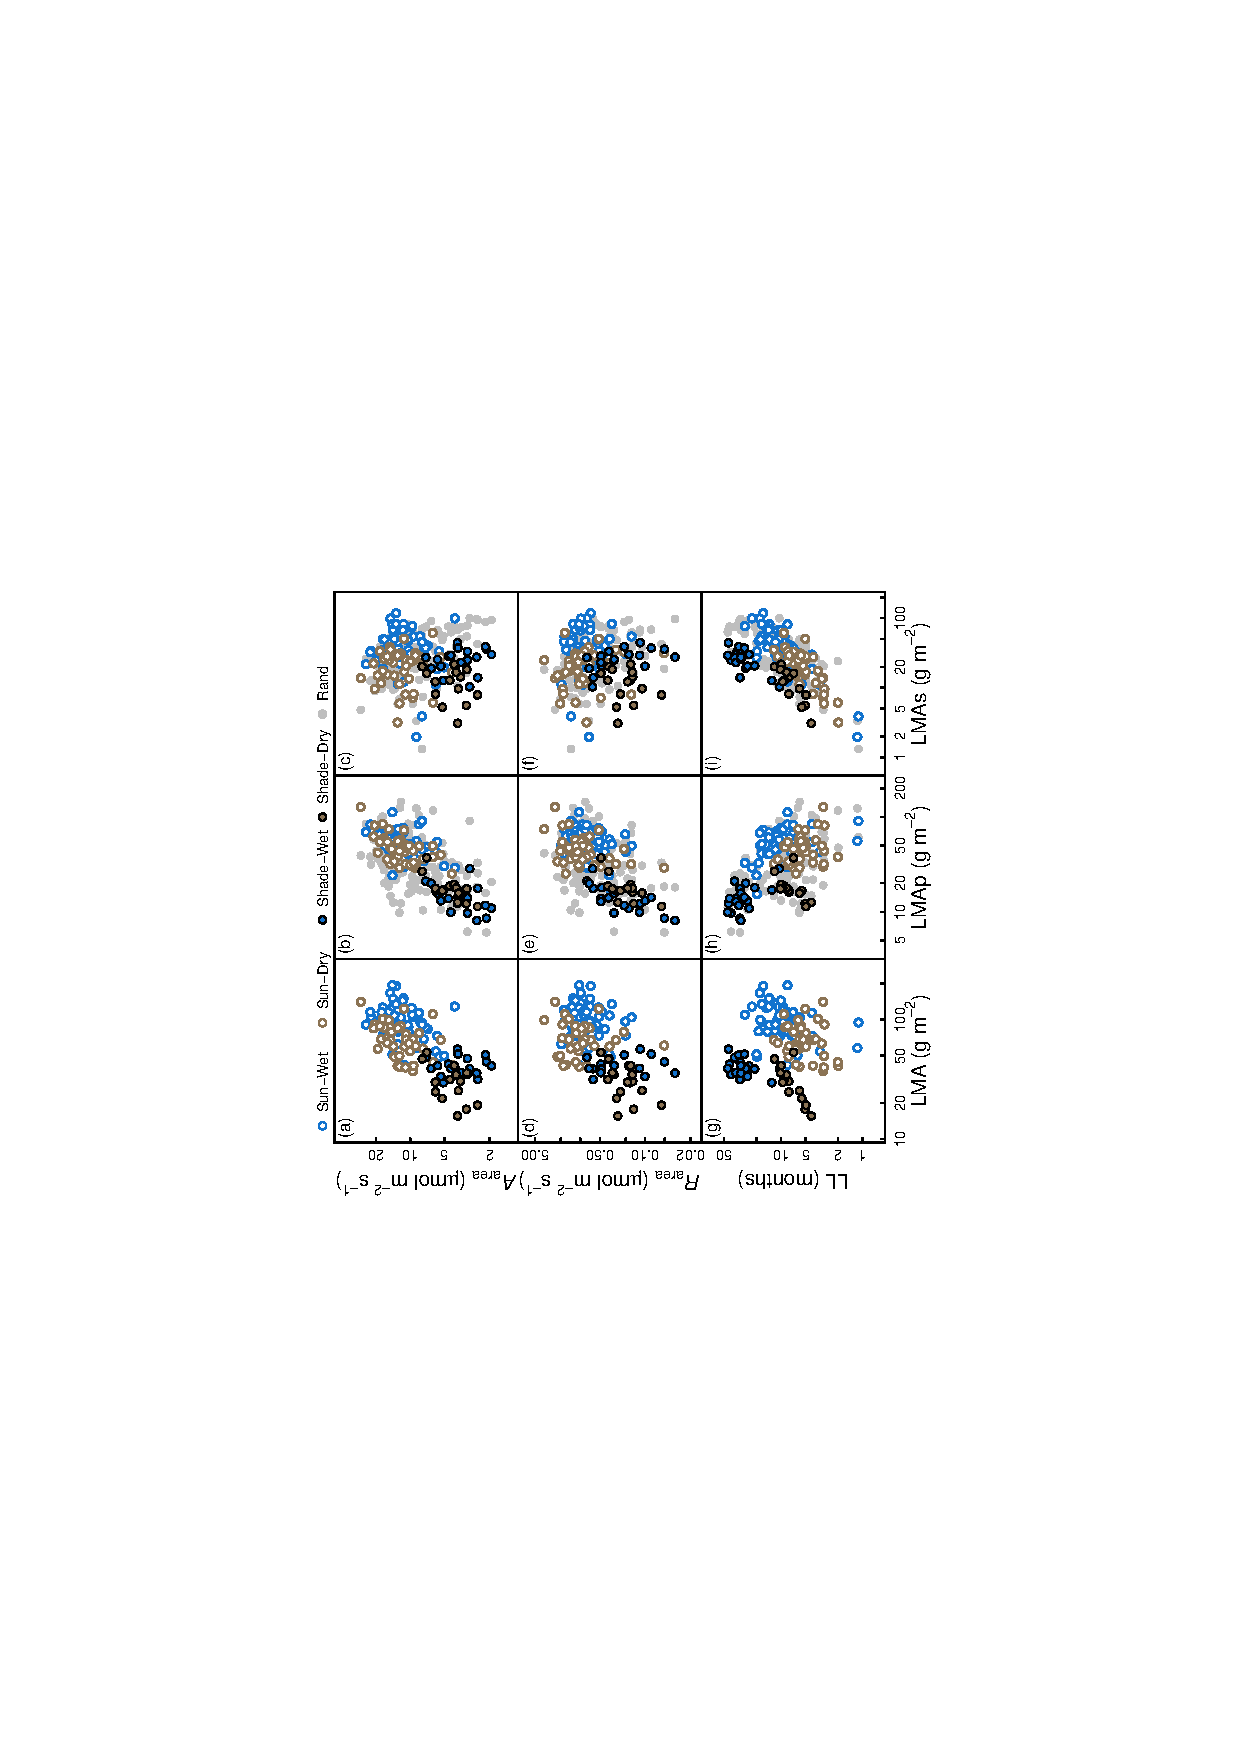
\includegraphics{../figs/ELE/PA_site.pdf}
%DIFDELCMD < %%%
%DIFDELCMD < \caption{%
{%DIFAUXCMD
%DIFDELCMD < \label{fig:PA-plot}%%%
\DIFdelFL{Observed and estimated leaf-trait relationships
in the Panama dataset. Estimates are from the Optimal LL Model with site
effects (Eq. }%DIFDELCMD < \eqref{eq:optLL} %%%
\DIFdelFL{and Notes S3). Details as in Fig.
\ref{fig:GL-plot}, except that in the randomized dataset shown here
(gray symbols), LMA was randomized within sites (wet and dry) across
canopy strata (sun and shade). Results for other LL models are
summarized in Table S3.}}
%DIFAUXCMD
%DIFDELCMD < \end{figure}
%DIFDELCMD <

%DIFDELCMD < \hypertarget{section-3}{%
%DIFDELCMD < \subparagraph{}%DIFDELCMD < \label{section-3}%%%
}
%DIFDELCMD <

%DIFDELCMD < \newpage
%DIFDELCMD <

%DIFDELCMD < \begin{figure}
%DIFDELCMD < \centering
%DIFDELCMD < \includegraphics{../figs/ELE/Fig3_simple.pdf}
%DIFDELCMD < %%%
%DIFDELCMD < \caption{%
{%DIFAUXCMD
%DIFDELCMD < \label{fig:LL-pre}%%%
\DIFdelFL{Observed vs.~predicted leaf lifespan (LL) in the
(a) Potential LL Model (Eq. 5) and (b) Optimal LL Model with site
effects (Eq. 13 and Notes S3). Predicted LL values are posterior means.
The dashed line indicates the 1:1 relationship. Gray symbols show
predicted LL values from 1 of 10 randomized LMA datasets for each model.
Pearson correlation coefficients are for predictions derived from the
observed datasets, and P-values (*** P \textless{} 0.001) are for the
null hypothesis of equal correlation in observed and randomized datasets
(see `Randomized LMA Datasets' in Methods for details). Results for
other LL models are reported in Table S4.}}
%DIFAUXCMD
%DIFDELCMD < \end{figure}
%DIFDELCMD <

%DIFDELCMD < \hypertarget{section-4}{%
%DIFDELCMD < \subparagraph{}%DIFDELCMD < \label{section-4}%%%
}
%DIFDELCMD <

%DIFDELCMD < \newpage
%DIFDELCMD <

%DIFDELCMD < \begin{figure}
%DIFDELCMD < \centering
%DIFDELCMD < \includegraphics{../figs/ELE/bar_cov.pdf}
%DIFDELCMD < %%%
%DIFDELCMD < \caption{%
{%DIFAUXCMD
%DIFDELCMD < \label{fig:bar-cov}%%%
\DIFdelFL{Percent of interspecific variation in leaf mass
per area (LMA) explained by photosynthetic and structural components of
LMA (LMAm and LMAs, respectively) for the global GLOPNET dataset (GL),
sun leaves in Panama (PA Sun), and shade leaves in Panama (PA Shade).
Variance was partitioned by applying Eq. 15 to posterior means of LMAm
and LMAs.}}
%DIFAUXCMD
%DIFDELCMD < \end{figure}
%DIFDELCMD <

%DIFDELCMD < \hypertarget{section-5}{%
%DIFDELCMD < \subparagraph{}%DIFDELCMD < \label{section-5}%%%
}
%DIFDELCMD <

%DIFDELCMD < \newpage
%DIFDELCMD <

%DIFDELCMD < \begin{figure}
%DIFDELCMD < \centering
%DIFDELCMD < \includegraphics{../figs/ELE/trim_all.pdf}
%DIFDELCMD < %%%
%DIFDELCMD < \caption{%
{%DIFAUXCMD
%DIFDELCMD < \label{fig:box-mean}%%%
\DIFdelFL{Boxplots comparing leaf mass per area (LMA) and
posterior means of photosynthetic and structural LMA components (LMAm
and LMAs, respectively) across deciduous (D) and evergreen (E) leaves in
the GLOPNET dataset (top), and across sites (wet and dry) and canopy
strata (sun and shade) in the Panama dataset (bottom). The center line
in each box indicates the median, upper and lower box edges indicate the
interquartile range, whiskers show 1.5 times the interquartile range,
and points are outliers. Groups sharing the same letters are not
significantly different (P \textgreater{} 0.05; t-tests). To isolate the
effects of intraspecific variation (i.e., plastic responses to light),
the Panama results shown here only include species for which both sun
and shade leaves were available. Qualitatively similar results were
obtained when all Panama species were included (Fig. S2). Note that the
vertical axis is on a log\textsubscript{10} scale.}}
%DIFAUXCMD
%DIFDELCMD < \end{figure}
%DIFDELCMD <

%DIFDELCMD < \hypertarget{section-6}{%
%DIFDELCMD < \subparagraph{}%DIFDELCMD < \label{section-6}%%%
}
%DIFDELCMD <

%DIFDELCMD < \newpage
%DIFDELCMD <

%DIFDELCMD < \begin{figure}
%DIFDELCMD < \centering
%DIFDELCMD < 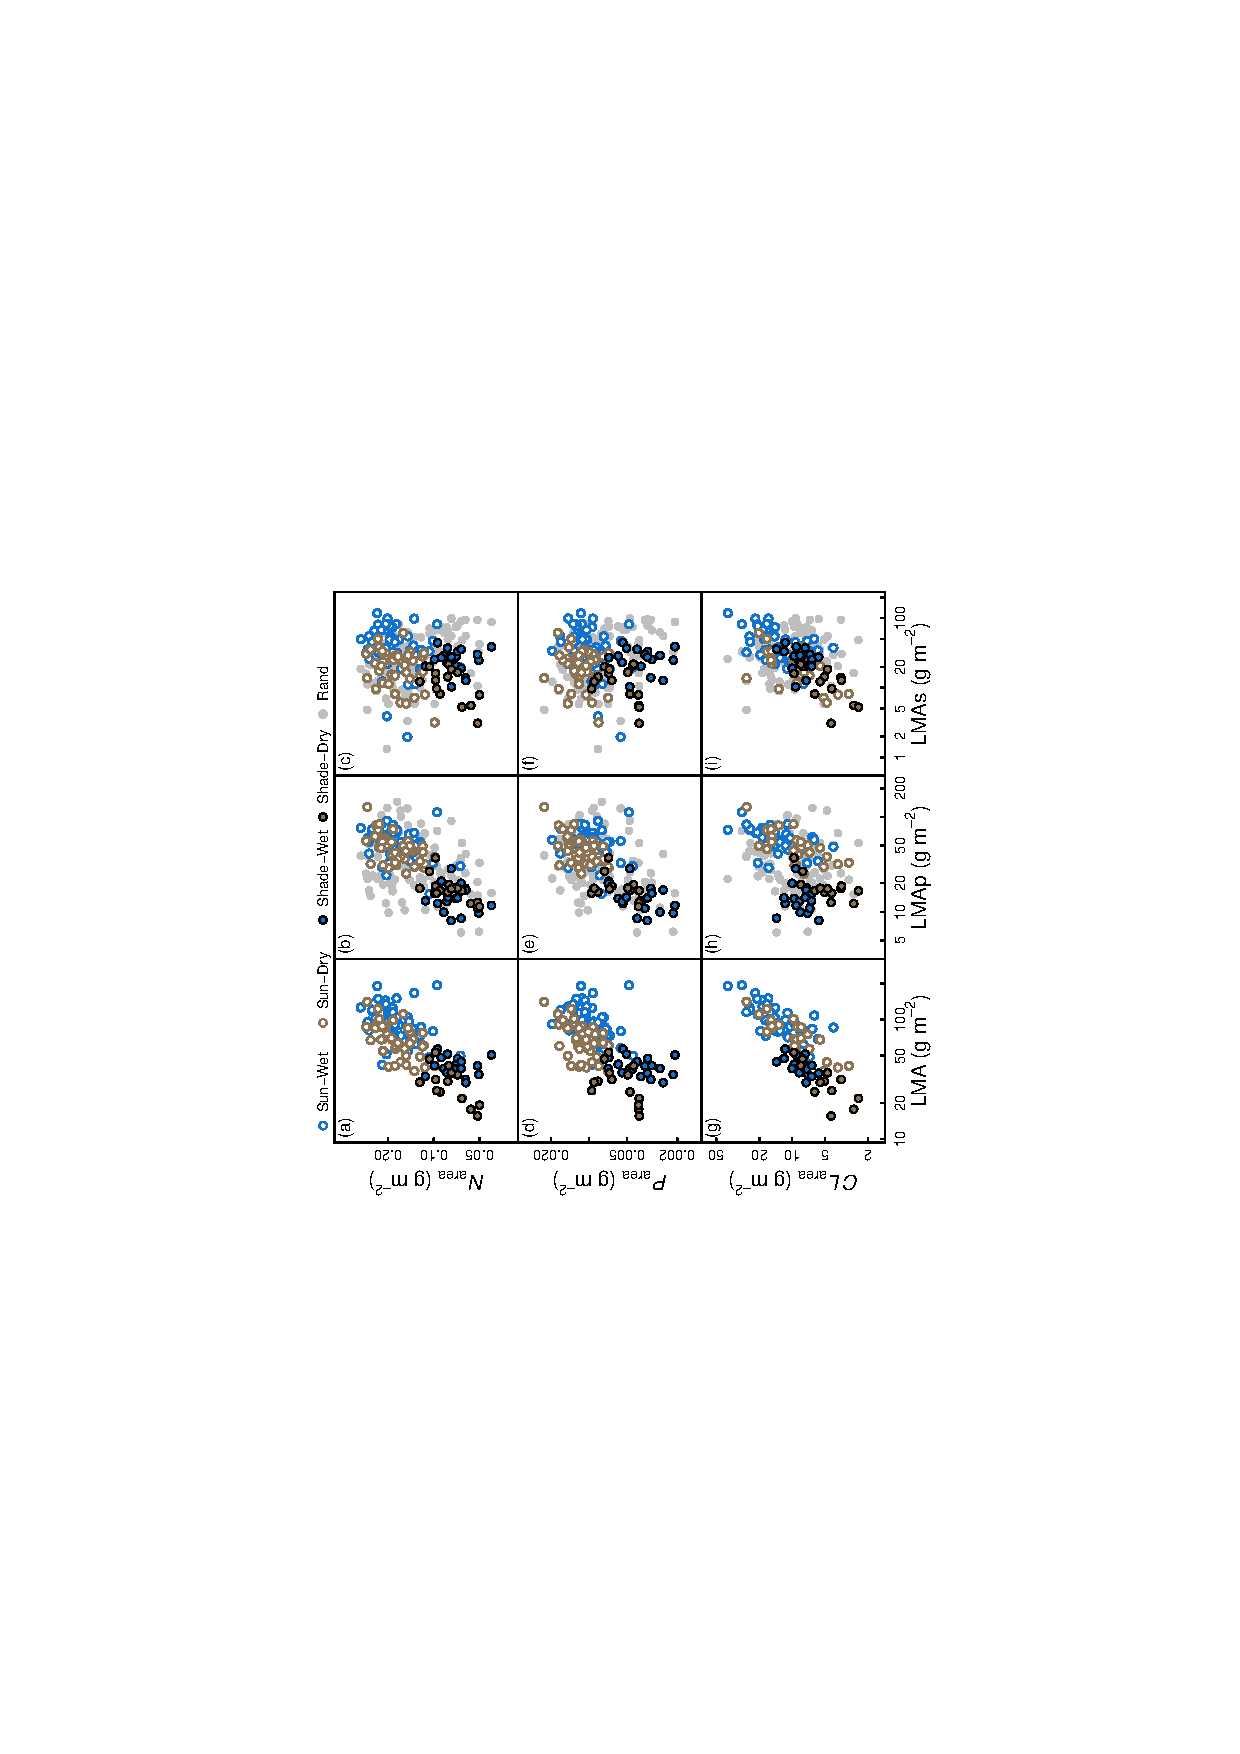
\includegraphics{../figs/ELE/NPC_site.pdf}
%DIFDELCMD < %%%
%DIFDELCMD < \caption{%
{%DIFAUXCMD
%DIFDELCMD < \label{fig:PA-NPC}%%%
\DIFdelFL{Measured traits related to photosynthesis and
metabolism traits (nitrogen and phosphorus per-unit leaf area;
}\emph{\DIFdelFL{N}}%DIFAUXCMD
\DIFdelFL{\textsubscript{area} and }\emph{\DIFdelFL{P}}%DIFAUXCMD
\DIFdelFL{\textsubscript{area}) are
strongly correlated with estimates (posterior means) of the
photosynthetic LMA component (LMAm), and a measured structural trait
(cellulose per-unit leaf area; }\emph{\DIFdelFL{CL}}%DIFAUXCMD
\DIFdelFL{\textsubscript{area}) is
strongly correlated with estimates of the structural LMA component
(LMAs) for the Panama dataset. Note that sun and shade leaves align
along a single relationship for }\emph{\DIFdelFL{CL}}%DIFAUXCMD
\DIFdelFL{\textsubscript{area} vs.~LMAs,
but not for }\emph{\DIFdelFL{CL}}%DIFAUXCMD
\DIFdelFL{\textsubscript{area} vs.~LMA or LMAm.
}\emph{\DIFdelFL{N}}%DIFAUXCMD
\DIFdelFL{\textsubscript{area}, }\emph{\DIFdelFL{P}}%DIFAUXCMD
\DIFdelFL{\textsubscript{area}, and
}\emph{\DIFdelFL{CL}}%DIFAUXCMD
\DIFdelFL{\textsubscript{area} data were not used to fit the models, and
are presented here as independent support for the model results.
Analogous results were obtained for }\emph{\DIFdelFL{N}}%DIFAUXCMD
\DIFdelFL{\textsubscript{area} and
}\emph{\DIFdelFL{P}}%DIFAUXCMD
\DIFdelFL{\textsubscript{area} vs.~LMALMAmm for GLOPNET (Fig. S3). Gray
symbols show 1 of 10 datasets in which LMA was randomized within sites
(wet and dry) across canopy strata (sun and shade). Others details as in
Fig. \ref{fig:GL-plot}. Results for other LL models are reported in
Table S3.}}
%DIFAUXCMD
%DIFDELCMD < \end{figure}
%DIFDELCMD <

%DIFDELCMD < \hypertarget{section-7}{%
%DIFDELCMD < \subparagraph{}%DIFDELCMD < \label{section-7}%%%
}
%DIFDELCMD <

%DIFDELCMD < \hypertarget{reference}{%
%DIFDELCMD < \section*{Reference}%DIFDELCMD < \label{reference}%%%
}
%DIFDELCMD < %%%
\addcontentsline{toc}{section}{\DIFdel{Reference}}
%DIFAUXCMD
%DIFDELCMD <

%DIFDELCMD < %%%
\DIFdelend \hypertarget{refs}{}
\leavevmode\hypertarget{ref-Akaike1973}{}%
Akaike, H. (1973). Information theory and an extension of the maximum
likelihood principle. In B. N. Petrov \& F. Csaki (Eds.), \emph{Second
international symposium on information theory} (pp. 267--281). Budapest:
Akadémiai Kiado.

\leavevmode\DIFdelbegin %DIFDELCMD < \hypertarget{ref-Alvarez2014}{}%%%
%DIF <
\DIFdel{Alvarez, I., Niemi, J., \& Simpson, M. (2014). Bayesian inference for a
covariance matrix. }\emph{\DIFdel{arXiv Preprint arXiv:1408.4050v2}}%DIFAUXCMD
\DIFdel{, 1--12.
doi:}%DIFDELCMD < \href{https://doi.org/10.1214/aos/1176348885}{10.1214/aos/1176348885}
%DIFDELCMD <

%DIFDELCMD < \leavevmode%%%
\DIFdelend \hypertarget{ref-Aranda2004}{}%
Aranda, I., Pardo, F., Gil, L., \& Pardos, J. A. (2004). Anatomical
basis of the change in leaf mass per area and nitrogen investment with
relative irradiance within the canopy of eight temperate tree species.
\emph{Acta Oecologica}, \emph{25}(3), 187--195.
doi:\href{https://doi.org/10.1016/j.actao.2004.01.003}{10.1016/j.actao.2004.01.003}

\leavevmode\hypertarget{ref-Bishop2006}{}%
Bishop, C. M. (2006). \emph{Pattern Recognition and Machine Learning}.
New York: Springer.

\leavevmode\DIFdelbegin %DIFDELCMD < \hypertarget{ref-Bonan2002}{}%%%
%DIF <
\DIFdel{Bonan, G. B., Levis, S., Kergoat, L., \& Oleson, K. W. (2002).
Landscapes as patches of plant functional types: An integrating concept
for climate and ecosystem models. }\emph{\DIFdel{Global Biogeochemical Cycles}}%DIFAUXCMD
\DIFdel{,
}%DIFDELCMD < \emph{16}(2)%%%
\DIFdel{, 5--1--5--23.
doi:}%DIFDELCMD < \href{https://doi.org/10.1029/2000GB001360}{10.1029/2000GB001360}
%DIFDELCMD <

%DIFDELCMD < \leavevmode%%%
\DIFdelend \hypertarget{ref-Carpenter2017}{}%
Carpenter, B., Gelman, A., Hoffman, M. D., Lee, D., Goodrich, B.,
Betancourt, M., \ldots{} Riddell, A. (2017). Stan : A Probabilistic
Programming Language. \emph{Journal of Statistical Software},
\emph{76}(1), 1--32.
doi:\href{https://doi.org/10.18637/jss.v076.i01}{10.18637/jss.v076.i01}

\leavevmode\DIFdelbegin %DIFDELCMD < \hypertarget{ref-Ellsworth1993}{}%%%
\DIFdelend \DIFaddbegin \hypertarget{ref-Evans2009}{}\DIFaddend %
\DIFdelbegin \DIFdel{Ellsworth, D. S., \& Reich, P. B. (1993). Canopy structure and vertical
patterns of photosynthesis and related leaf traits in a deciduous
forest. }\emph{\DIFdel{Oecologia}}%DIFAUXCMD
\DIFdelend \DIFaddbegin \DIFadd{Evans}\DIFaddend , \DIFdelbegin %DIFDELCMD < \emph{96}(2)%%%
\DIFdelend \DIFaddbegin \DIFadd{J. R.}\DIFaddend , \DIFdelbegin \DIFdel{169--178.
doi:}%DIFDELCMD < \href{https://doi.org/10.1007/BF00317729}{10.1007/BF00317729}
%DIFDELCMD <

%DIFDELCMD < \leavevmode\hypertarget{ref-Evans2008}{}%%%
%DIF <
\DIFdel{Evans, B. J. , McGuire, J.A., Brown}\DIFdelend \DIFaddbegin \DIFadd{Kaldenhoff}\DIFaddend , R.\DIFdelbegin \DIFdel{M., Andayani, N}\DIFdelend \DIFaddbegin \DIFadd{, Genty, B}\DIFaddend ., \& \DIFdelbegin \DIFdel{Supriatna, J. (2008).
A coalescent framework for comparing alternative models of
population structure with genetic data: evolution of Celebes toads. }\DIFdelend \DIFaddbegin \DIFadd{Terashima, I. (2009).
Resistances along the CO2 diffusion pathway inside leaves. }\DIFaddend \emph{\DIFdelbegin \DIFdel{Biology Letters}\DIFdelend \DIFaddbegin \DIFadd{Journal
of Experimental Botany}\DIFaddend }, \DIFdelbegin %DIFDELCMD < \emph{4}(4)%%%
\DIFdel{, 430--433}\DIFdelend \DIFaddbegin \emph{60}(8)\DIFadd{, 2235--2248}\DIFaddend .
doi:\DIFdelbegin %DIFDELCMD < \href{https://doi.org/10.1098/rsbl.2008.0166}{10.1098/rsbl.2008.0166}
%DIFDELCMD < %%%
\DIFdelend \DIFaddbegin \href{https://doi.org/10.1093/jxb/erp117}{10.1093/jxb/erp117}
\DIFaddend

\leavevmode\hypertarget{ref-Gelman2006}{}%
Gelman, A., \& Hill, J. (2006). \emph{Multilevel regression} (pp.
235--236).
doi:\href{https://doi.org/10.1017/CBO9780511790942.014}{10.1017/CBO9780511790942.014}

\leavevmode\hypertarget{ref-Gelman2014}{}%
Gelman, A., Hwang, J., \& Vehtari, A. (2014). Understanding predictive
information criteria for Bayesian models. \emph{Statistics and
Computing}, \emph{24}(6), 997--1016.
doi:\href{https://doi.org/10.1007/s11222-013-9416-2}{10.1007/s11222-013-9416-2}

\leavevmode\DIFdelbegin %DIFDELCMD < \hypertarget{ref-Gotelli2002}{}%%%
%DIF <
\DIFdel{Gotelli, N. J., \& Rohde, K. (2002). Co-occurrence of ectoparasites of
marine fishes: A null model analysis. }\emph{\DIFdel{Ecology Letters}}%DIFAUXCMD
\DIFdel{,
}%DIFDELCMD < \emph{5}(1)%%%
\DIFdel{, 86--94.
doi:}%DIFDELCMD < \href{https://doi.org/10.1046/j.1461-0248.2002.00288.x}{10.1046/j.1461-0248.2002.00288.x}
%DIFDELCMD <

%DIFDELCMD < \leavevmode%%%
\DIFdelend \hypertarget{ref-John2017}{}%
John, G. P., Scoffoni, C., Buckley, T. N., Villar, R., Poorter, H., \&
Sack, L. (2017). The anatomical and compositional basis of leaf mass per
area. \emph{Ecology Letters}, \emph{20}(4), 412--425.
doi:\href{https://doi.org/10.1111/ele.12739}{10.1111/ele.12739}

\leavevmode\DIFdelbegin %DIFDELCMD < \hypertarget{ref-Kenzo2006}{}%%%
%DIF <
\DIFdel{Kenzo, T., Ichie, T., Watanabe, Y., Yoneda, R., Ninomiya, I., \& Koike,
T. (2006). Changes in photosynthesis and leaf characteristics with tree
height in five dipterocarp species in a tropical rain forest. }\emph{\DIFdel{Tree
Physiology}}%DIFAUXCMD
\DIFdel{, }%DIFDELCMD < \emph{26}(7)%%%
\DIFdel{, 865--873.
doi:}%DIFDELCMD < \href{https://doi.org/10.1093/treephys/26.7.865}{10.1093/treephys/26.7.865}
%DIFDELCMD <

%DIFDELCMD < \leavevmode%%%
\DIFdelend \hypertarget{ref-Kikuzawa1991}{}%
Kikuzawa, K. (1991). A Cost-Benefit Analysis of Leaf Habit and Leaf
Longevity of Trees and Their Geographical. \emph{The American
Naturalist}, \emph{138}(5), 1250--1263.
doi:\href{https://doi.org/10.2307/2462519}{10.2307/2462519}

\leavevmode\hypertarget{ref-Kikuzawa2013}{}%
Kikuzawa, K., Onoda, Y., Wright, I. J., \& Reich, P. B. (2013).
Mechanisms underlying global temperature-related patterns in leaf
longevity. \emph{Global Ecology and Biogeography}, \emph{22}(8),
982--993.
doi:\href{https://doi.org/10.1111/geb.12042}{10.1111/geb.12042}

\leavevmode\hypertarget{ref-Kikuzawa2004}{}%
Kikuzawa, K., Shirakawa, H., Suzuki, M., \& Umeki, K. (2004). Mean labor
time of a leaf. \emph{Ecological Research}, \emph{19}(4), 365--374.
doi:\href{https://doi.org/10.1111/j.1440-1703.2004.00657.x}{10.1111/j.1440-1703.2004.00657.x}

\leavevmode\hypertarget{ref-Kitajima2013}{}%
Kitajima, K., Cordero, R. A., \& Wright, S. J. (2013). Leaf life span
spectrum of tropical woody seedlings: Effects of light and ontogeny and
consequences for survival. \emph{Annals of Botany}, \emph{112}(4),
685--699.
doi:\href{https://doi.org/10.1093/aob/mct036}{10.1093/aob/mct036}

\leavevmode\hypertarget{ref-Kitajima2012}{}%
Kitajima, K., Llorens, A. M., Stefanescu, C., Timchenko, M. V., Lucas,
P. W., \& Wright, S. J. (2012). How cellulose-based leaf toughness and
lamina density contribute to long leaf lifespans of shade-tolerant
species. \emph{New Phytologist}, \emph{195}(3), 640--652.
doi:\href{https://doi.org/10.1111/j.1469-8137.2012.04203.x}{10.1111/j.1469-8137.2012.04203.x}

\leavevmode\hypertarget{ref-Kitajima2010}{}%
Kitajima, K., \& Poorter, L. (2010). Tissue-level leaf toughness, but
not lamina thickness, predicts sapling leaf lifespan and shade tolerance
of tropical tree species. \emph{New Phytologist}, \emph{186}(3),
708--721.
doi:\href{https://doi.org/10.1111/j.1469-8137.2010.03212.x}{10.1111/j.1469-8137.2010.03212.x}

\leavevmode\hypertarget{ref-Kitajima2016}{}%
Kitajima, K., Wright, S. J., \& Westbrook, J. W. (2016). Leaf cellulose
density as the key determinant of inter- and intra-specific variation in
leaf fracture toughness in a species-rich tropical forest.
\emph{Interface Focus}, \emph{6}(3), 20150100.
doi:\href{https://doi.org/10.1098/rsfs.2015.0100}{10.1098/rsfs.2015.0100}

\leavevmode\DIFdelbegin %DIFDELCMD < \hypertarget{ref-Lewandowski2009}{}%%%
\DIFdelend \DIFaddbegin \hypertarget{ref-Kleyer2012}{}\DIFaddend %
\DIFdelbegin \DIFdel{Lewandowski, D., Kurowicka, D., \& Joe, H.(2009). Generating random
correlation matrices based on vines and extended onion method.
}\DIFdelend \DIFaddbegin \DIFadd{Kleyer, M., Dray, S., Bello, F., Lepš, J., Pakeman, R. J., Strauss, B.,
\ldots{} Lavorel, S. (2012). Assessing species and community functional
responses to environmental gradients: Which multivariate methods?
}\DIFaddend \emph{Journal of \DIFdelbegin \DIFdel{Multivariate Analysis}\DIFdelend \DIFaddbegin \DIFadd{Vegetation Science}\DIFaddend }, \DIFdelbegin %DIFDELCMD < \emph{100}(9)%%%
\DIFdel{, 1989--2001}\DIFdelend \DIFaddbegin \emph{23}(5)\DIFadd{, 805--821}\DIFaddend .
doi:\DIFdelbegin %DIFDELCMD < \href{https://doi.org/10.1016/j.jmva.2009.04.008}{10.1016/j.jmva.2009.04.008}
%DIFDELCMD < %%%
\DIFdelend \DIFaddbegin \href{https://doi.org/10.1111/j.1654-1103.2012.01402.x}{10.1111/j.1654-1103.2012.01402.x}
\DIFaddend

\leavevmode\hypertarget{ref-Lloyd2013}{}%
Lloyd, J., Bloomfield, K., Domingues, T. F., \& Farquhar, G. D. (2013).
Photosynthetically relevant foliar traits correlating better on a mass
vs an area basis: Of ecophysiological relevance or just a case of
mathematical imperatives and statistical quicksand? \emph{New
Phytologist}, \emph{199}(2), 311--321.
doi:\href{https://doi.org/10.1111/nph.12281}{10.1111/nph.12281}

\leavevmode\hypertarget{ref-Lusk2010}{}%
Lusk, C. H., Onoda, Y., Kooyman, R., \& Gutiérrez-Girón, A. (2010).
Reconciling species-level vs plastic responses of evergreen leaf
structure to light gradients: Shade leaves punch above their weight.
\emph{New Phytologist}, \emph{186}(2), 429--438.
doi:\href{https://doi.org/10.1111/j.1469-8137.2010.03202.x}{10.1111/j.1469-8137.2010.03202.x}

\leavevmode\hypertarget{ref-Lusk2008}{}%
Lusk, C. H., Reich, P. B., Montgomery, R. A., Ackerly, D. D., \&
Cavender-Bares, J. (2008). Why are evergreen leaves so contrary about
shade? \emph{Trends in Ecology and Evolution}, \emph{23}(6), 299--303.
doi:\href{https://doi.org/10.1016/j.tree.2008.02.006}{10.1016/j.tree.2008.02.006}

\leavevmode\hypertarget{ref-Niinemets2015}{}%
Niinemets, Ü., Keenan, T. F., \& Hallik, L. (2015). A worldwide analysis
of within-canopy variations in leaf structural, chemical and
physiological traits across plant functional types. \emph{New
Phytologist}, \emph{205}(3), 973--993.
doi:\href{https://doi.org/10.1111/nph.13096}{10.1111/nph.13096}

\leavevmode\hypertarget{ref-Onoda2008}{}%
Onoda, Y., Schieving, F., \& Anten, N. P. (2008). Effects of light and
nutrient availability on leaf mechanical properties of Plantago major: A
conceptual approach. \emph{Annals of Botany}, \emph{101}(5), 727--736.
doi:\href{https://doi.org/10.1093/aob/mcn013}{10.1093/aob/mcn013}

\leavevmode\hypertarget{ref-Onoda2017}{}%
Onoda, Y., Wright, I. J., Evans, J. R., Hikosaka, K., Kitajima, K.,
Niinemets, Ü., \ldots{} Westoby, M. (2017). Physiological and structural
tradeoffs underlying the leaf economics spectrum. \emph{New
Phytologist}, \emph{214}(4), 1447--1463.
doi:\href{https://doi.org/10.1111/nph.14496}{10.1111/nph.14496}

\leavevmode\DIFdelbegin %DIFDELCMD < \hypertarget{ref-Osada2001}{}%%%
\DIFdelend \DIFaddbegin \hypertarget{ref-Osnas2018}{}\DIFaddend %
\DIFdelbegin \DIFdel{Osada, N. , Takeda, H., Furukawa, }\DIFdelend \DIFaddbegin \DIFadd{Osnas, J. L. D., Katabuchi, M., Kitajima, K., Wright, S. J., Reich, P.
B., Van Bael, S. }\DIFaddend A., \DIFdelbegin \DIFdel{\& Awang, M. (2001). Leaf dynamics
and maintenance of tree crowns in a malaysian rain forest stand.
}\emph{\DIFdel{Journal of Ecology}}%DIFAUXCMD
\DIFdel{, }%DIFDELCMD < \emph{89}(5)%%%
\DIFdel{, 774--782. doi:}%DIFDELCMD < \href{https://doi.org/10.1046/j.0022-0477.2001.00590.x}{10.1046/j.0022-0477.2001.00590.x}
%DIFDELCMD < %%%
\DIFdelend \DIFaddbegin \DIFadd{\ldots{} Lichstein, J. W. (2018). Divergent drivers
of leaf trait variation within species, among species, and among
functional groups. }\emph{\DIFadd{Proceedings of the National Academy of Sciences
of the United States of America}}\DIFadd{, 201803989.
doi:}\href{https://doi.org/10.1073/pnas.1803989115}{10.1073/pnas.1803989115}
\DIFaddend

\leavevmode\hypertarget{ref-Osnas2013}{}%
Osnas, J. L. D., Lichstein, J. W., Reich, P. B., \& Pacala, S. W.
(2013). Global leaf trait relationships: Mass, area, and the leaf
economics spectrum. \emph{Science}, \emph{340}(6133), 741--744.
doi:\href{https://doi.org/10.1126/science.1231574}{10.1126/science.1231574}

\leavevmode\hypertarget{ref-Poorter2006b}{}%
Poorter, H., Pepin, S., Rijkers, T., De Jong, Y., Evans, J. R., \&
Körner, C. (2006). Construction costs, chemical composition and payback
time of high- and low-irradiance leaves. \emph{Journal of Experimental
Botany}, \emph{57}(2 SPEC. ISS.), 355--371.
doi:\href{https://doi.org/10.1093/jxb/erj002}{10.1093/jxb/erj002}

\leavevmode\hypertarget{ref-Reich2014}{}%
Reich, P. B. (2014). The world-wide 'fast-slow' plant economics
spectrum: A traits manifesto. \emph{Journal of Ecology}, \emph{102}(2),
275--301.
doi:\href{https://doi.org/10.1111/1365-2745.12211}{10.1111/1365-2745.12211}

\leavevmode\DIFdelbegin %DIFDELCMD < \hypertarget{ref-Reich1997}{}%%%
%DIF <
\DIFdel{Reich, P. B., Walters, M. B., \& Ellsworth, D. S. (1997). From tropics
to tundra: Global convergence in plant functioning. }\emph{\DIFdel{Proceedings of
the National Academy of Sciences}}%DIFAUXCMD
\DIFdel{, }%DIFDELCMD < \emph{94}(25)%%%
\DIFdel{, 13730--13734.
doi:}%DIFDELCMD < \href{https://doi.org/10.1073/pnas.94.25.13730}{10.1073/pnas.94.25.13730}
%DIFDELCMD <

%DIFDELCMD < \leavevmode%%%
\DIFdelend \hypertarget{ref-Roderick1999}{}%
Roderick, M. L., Berry, S. L., Noble, I. R., \& Farquhar, G. D. (1999).
A theoretical approach to linking the composition and morphology with
the function of leaves. \emph{Functional Ecology}, \emph{13}(5),
683--695.
doi:\href{https://doi.org/10.1046/j.1365-2435.1999.00368.x}{10.1046/j.1365-2435.1999.00368.x}

\leavevmode\DIFdelbegin %DIFDELCMD < \hypertarget{ref-Russo2016}{}%%%
%DIF <
\DIFdel{Russo, S. E., \& Kitajima, K. (2016). The Ecophysiology of Leaf Lifespan
in Tropical Forests: Adaptive and Plastic Responses to Environmental
Heterogeneity. In G. Goldstein \& S. L. Santiago (Eds.), }\emph{\DIFdel{Tropical
tree physiology}} %DIFAUXCMD
\DIFdel{(pp. 357--383). Cham: Springer International
Publishing.
doi:}%DIFDELCMD < \href{https://doi.org/10.1007/978-3-319-27422-5_17}{10.1007/978-3-319-27422-5\_17}
%DIFDELCMD <

%DIFDELCMD < \leavevmode%%%
\DIFdelend \hypertarget{ref-Scheiter2013}{}%
Scheiter, S., Langan, L., \& Higgins, S. I. (2013). Next-generation
dynamic global vegetation models: Learning from community ecology.
\emph{New Phytologist}, \emph{198}(3), 957--969.
doi:\href{https://doi.org/10.1111/nph.12210}{10.1111/nph.12210}

\leavevmode\hypertarget{ref-Shipley2006}{}%
Shipley, B., Lechowicz, M. J., Wright, I., \& Reich, P. B. (2006).
Fundamental trade-offs generating the worldwide leaf economics spectrum.
\emph{Ecology}, \emph{87}(3), 535--541.
doi:\href{https://doi.org/10.1890/05-1051}{10.1890/05-1051}

\leavevmode\hypertarget{ref-Spiegelhalter2002}{}%
Spiegelhalter, D. J., Best, N. G., Carlin, B. P., \& Van Der Linde, A.
(2002). Bayesian measures of model complexity and fit. \emph{Journal of
the Royal Statistical Society. Series B: Statistical Methodology},
\emph{64}(4), 583--616.
doi:\href{https://doi.org/10.1111/1467-9868.00353}{10.1111/1467-9868.00353}

\leavevmode\hypertarget{ref-Terashima2011}{}%
Terashima, I., Hanba, Y. T., Tholen, D., \& Niinemets, U. (2011). Leaf
Functional Anatomy in Relation to Photosynthesis. \emph{Plant
Physiology}, \emph{155}(1), 108--116.
doi:\href{https://doi.org/10.1104/pp.110.165472}{10.1104/pp.110.165472}

\leavevmode\hypertarget{ref-Villar2001}{}%
Villar, R., \& Merino, J. (2001). Comparison of leaf construction costs
in woody species with differing leaf-spans in contrasting ecosystems.
\emph{New Phytologist}, \emph{151}, 213--226.
doi:\href{https://doi.org/10.1046/j.1469-8137.2001.00147.x/pdf}{10.1046/j.1469-8137.2001.00147.x/pdf}

\leavevmode\hypertarget{ref-Watanabe2010}{}%
Watanabe, S. (2010). Asymptotic Equivalence of Bayes Cross Validation
and Widely Applicable Information Criterion in Singular Learning Theory.
\emph{The Journal of Machine Learning Research}, \emph{11}, 3571--3594.
Retrieved from \url{http://arxiv.org/abs/1004.2316}

\leavevmode\DIFdelbegin %DIFDELCMD < \hypertarget{ref-Westoby2006}{}%%%
\DIFdelend \DIFaddbegin \hypertarget{ref-Westoby2013}{}\DIFaddend %
Westoby, M.\DIFdelbegin \DIFdel{(2006). Phylogenetic ecology at world scale, a new fusion
between ecology and evolution.
}\emph{\DIFdel{Ecology}}%DIFAUXCMD
\DIFdel{, }\emph{\DIFdel{87}}%DIFAUXCMD
\DIFdel{(7 SUPPL.)}\DIFdelend \DIFaddbegin \DIFadd{, Reich, P. B., \& Wright, I. J. (2013). Understanding
ecological variation across species: Area-based vs mass-based expression
of leaf traits. }\emph{\DIFadd{New Phytologist}}\DIFadd{, }\emph{199}(2)\DIFaddend , \DIFdelbegin \DIFdel{S163-----S166}\DIFdelend \DIFaddbegin \DIFadd{322--323.
doi:}\href{https://doi.org/10.1111/nph.12345}{10.1111/nph.12345}

\leavevmode\hypertarget{ref-Westoby2006a}{}%DIF >
\DIFadd{Westoby, M., \& Wright, I. J. (2006)}\DIFaddend . \DIFaddbegin \DIFadd{Land-plant ecology on the basis of
functional traits. }\emph{\DIFadd{Trends in Ecology and Evolution}}\DIFadd{, }\emph{21}(5)\DIFadd{,
261--268.
}\DIFaddend doi:\DIFdelbegin %DIFDELCMD < \href{https://doi.org/10.1890/0012-9658(2006)87\%5B163:PEAWSA\%5D2.0.CO;2}{10.1890/0012-9658(2006)87{[}163:PEAWSA{]}2.0.CO;2}
%DIFDELCMD < %%%
\DIFdelend \DIFaddbegin \href{https://doi.org/10.1016/j.tree.2006.02.004}{10.1016/j.tree.2006.02.004}
\DIFaddend

\leavevmode\hypertarget{ref-Williams1989}{}%
Williams, K., Field, C. B., \& Mooney, H. A. (1989). Relationships Among
Leaf Construction Cost, Leaf Longevity, and Light Environment in
Rain-Forest Plants of the Genus Piper. \emph{The American Naturalist},
\emph{133}(2), 198--211.
doi:\href{https://doi.org/10.1086/284910}{10.1086/284910}

\leavevmode\hypertarget{ref-Wright2004a}{}%
Wright, I. J., Reich, P. B., Westoby, M., Ackerly, D. D., Baruch, Z.,
Bongers, F., \ldots{} Villar, R. (\DIFdelbegin \DIFdel{2004}\DIFdelend \DIFaddbegin \DIFadd{2004a}\DIFaddend ). The worldwide leaf economics
spectrum. \emph{Nature}, \emph{428}(6985), 821--827.
doi:\href{https://doi.org/10.1038/nature02403}{10.1038/nature02403}

\leavevmode\hypertarget{ref-Wright2004}{}%
Wright, S. J., Calderón, O., Hernandéz, A., \& Paton, S. (\DIFdelbegin \DIFdel{2004}\DIFdelend \DIFaddbegin \DIFadd{2004b}\DIFaddend ). Are
lianas increasing in importance in tropical forests? A 17-year record
from panama. \emph{Ecology}, \emph{85}(2), 484--489.
doi:\href{https://doi.org/10.1890/02-0757}{10.1890/02-0757}

\leavevmode\hypertarget{ref-Wright2003}{}%
Wright, S. J., Horlyck, V., Basset, Y., Barrios, H., Bethancourt, A.,
Bohlman, S., \ldots{} Zotz, G. (2003). Tropical Canopy Biology Program,
Republic of Panama. In Y. Basset, V. Horlyck, \& S. J. Wright (Eds.),
\emph{Studying forest canopies from above: The international canopy
crane network} (pp. 137--155). Panama.

\leavevmode\hypertarget{ref-Wullschleger2014}{}%
Wullschleger, S. D., Epstein, H. E., Box, E. O., Euskirchen, E. S.,
Goswami, S., Iversen, C. M., \ldots{} Xu, X. (2014). Plant functional
types in Earth system models: Past experiences and future directions for
application of dynamic vegetation models in high-latitude ecosystems.
\emph{Annals of Botany}, \emph{114}(1), 1--16.
doi:\href{https://doi.org/10.1093/aob/mcu077}{10.1093/aob/mcu077}
\DIFaddbegin

\newpage

\hypertarget{figures}{%
\section{Figures}\label{figures}}

\begin{figure}
\centering
\includegraphics{LMAps_main_re_files/figure-latex/GLplt-1.pdf}
\caption{\label{fig:GLplt}\DIFaddFL{Observed and estimated leaf-trait relationships in
the global GLOPNET dataset. Leaf life span (LL), net photosynthetic rate
per unit leaf area (}\emph{\DIFaddFL{A}}\DIFaddFL{\textsubscript{area}), and dark respiration
rate per unit leaf area (}\emph{\DIFaddFL{R}}\DIFaddFL{\textsubscript{area}) are plotted
against observed LMA and estimates (posterior means) of photosynthetic
and structural LMA components (LMAm and LMAs, respectively). Gray
symbols show 1 of 10 randomized datasets, in which LMA was randomized
among all leaves in the GLOPNET dataset we analyzed (which includes all
leaves for which LMA, }\emph{\DIFaddFL{A}}\DIFaddFL{\textsubscript{area},
}\emph{\DIFaddFL{R}}\DIFaddFL{\textsubscript{area}, and LL were available). Pearson
correlation coefficients are for observed LMA (left column) and
posterior means of LMAm (middle column) and LMAs (right column). Signs
of inequality indicates }\emph{\DIFaddFL{r\textsubscript{obs}}} \DIFaddFL{are significant
(against null hypothesis of zero correlation) and they do not overlap
}\emph{\DIFaddFL{r\textsubscript{rand}}} \DIFaddFL{(see Fig. 1).}}
\end{figure}

\newpage

\hypertarget{section}{%
\section{}\label{section}}

\begin{figure}
\centering
\includegraphics{LMAps_main_re_files/figure-latex/PAplt-1.pdf}
\caption{\label{fig:PAplt}\DIFaddFL{Observed and estimated leaf-trait relationships in
the Panama dataset. Estimates are from the Optimal LL Model with site
effects (Eq. 13 and Notes S3). Details as in Fig. GL. Results for other
LL models are summarized in Table SX.}}
\end{figure}

\newpage

\hypertarget{section-1}{%
\section{}\label{section-1}}

\begin{figure}
\centering
\includegraphics{LMAps_main_re_files/figure-latex/LLplt-1.pdf}
\caption{\label{fig:LLplt}\DIFaddFL{Observed vs.~predicted leaf lifespan (LL) in the
(a) Potential LL Model (Eq. 5) and (b) Optimal LL Model with site
effects (Eq. 13 and Notes S3). Predicted LL values are posterior means.
The dashed line indicates the 1:1 relationship. Gray symbols show
predicted LL values from 1 of 10 randomized LMA datasets for each model.
Pearson correlation coefficients are for predictions derived from the
observed datasets, and tested against the null hypothesis of equal
correlation in observed and randomized datasets (see Fig. 1). Results
for other LL models are reported in Table S4.}}
\end{figure}

\newpage

\hypertarget{section-2}{%
\section{}\label{section-2}}

\begin{figure}
\centering
\includegraphics{LMAps_main_re_files/figure-latex/covplt-1.pdf}
\caption{\label{fig:covplt}\DIFaddFL{Percent of interspecific variation in leaf mass
per area (LMA) explained by photosynthetic and structural components of
LMA (LMAm and LMAs, respectively) for the global GLOPNET dataset (GL),
sun leaves in Panama (PA Sun), and shade leaves in Panama (PA Shade).
Variance was partitioned by applying Eq. 15 to posterior means of LMAm
and LMAs}}
\end{figure}

\newpage

\hypertarget{section-3}{%
\section{}\label{section-3}}

\begin{figure}
\centering
\includegraphics{LMAps_main_re_files/figure-latex/boxplt-1.pdf}
\caption{\label{fig:boxplt}\DIFaddFL{Boxplots comparing leaf mass per area (LMA) and
posterior means of photosynthetic and structural LMA components (LMAm
and LMAs, respectively) across deciduous (D) and evergreen (E) leaves in
the GLOPNET dataset (top), and across sites (wet and dry) and canopy
strata (sun and shade) in the Panama dataset (bottom). The center line
in each box indicates the median, upper and lower box edges indicate the
interquartile range, whiskers show 1.5 times the interquartile range,
and points are outliers. Groups sharing the same letters are not
significantly different (P \textgreater{} 0.05; t-tests). To isolate the
effects of intraspecific variation (i.e., plastic responses to light),
the Panama results shown here only include species for which both sun
and shade leaves were available. Qualitatively similar results were
obtained when all Panama species were included (Fig. S2). Note that the
vertical axis is on a log\textsubscript{10} scale.}}
\end{figure}

\newpage

\hypertarget{section-4}{%
\section{}\label{section-4}}

\begin{figure}
\centering
\includegraphics{LMAps_main_re_files/figure-latex/PA-NPC-1.pdf}
\caption{\label{fig:PA-NPC}\DIFaddFL{Measured traits related to photosynthesis and
metabolism traits (nitrogen and phosphorus per-unit leaf area;
}\emph{\DIFaddFL{N}}\DIFaddFL{\textsubscript{area} and }\emph{\DIFaddFL{P}}\DIFaddFL{\textsubscript{area}) are
strongly correlated with estimates (posterior means) of the
photosynthetic LMA component (LMAm), and a measured structural trait
(cellulose per-unit leaf area; }\emph{\DIFaddFL{CL}}\DIFaddFL{\textsubscript{area}) is
strongly correlated with estimates of the structural LMA component
(LMAs) for the Panama dataset. Note that sun and shade leaves align
along a single relationship for }\emph{\DIFaddFL{CL}}\DIFaddFL{\textsubscript{area} vs.~LMAs,
but not for }\emph{\DIFaddFL{CL}}\DIFaddFL{\textsubscript{area} vs.~LMA or LMAm.
}\emph{\DIFaddFL{N}}\DIFaddFL{\textsubscript{area}, }\emph{\DIFaddFL{P}}\DIFaddFL{\textsubscript{area}, and
}\emph{\DIFaddFL{CL}}\DIFaddFL{\textsubscript{area} data were not used to fit the models, and
are presented here as independent support for the model results.
Analogous results were obtained for }\emph{\DIFaddFL{N}}\DIFaddFL{\textsubscript{area} and
}\emph{\DIFaddFL{P}}\DIFaddFL{\textsubscript{area} vs.~LMAm for GLOPNET (Fig. S3). Gray
symbols show 1 of 10 datasets in which LMA was randomized within sites
(wet and dry) across canopy strata (sun and shade). Others details as in
Fig. GL. Results for other LL models are reported in Table S3.}}
\end{figure}
\DIFaddend


\end{document}
